\documentclass[aps,
 twocolumn,
superscriptaddress,notitlepage]{revtex4-1}
\usepackage{graphicx}
\usepackage{bm}
\usepackage{amsmath}
\usepackage{amsfonts}
\usepackage{amssymb}
\usepackage{array}
\usepackage{xcolor}
\usepackage{dcolumn}
\usepackage{longtable}
\usepackage{hyperref}
\usepackage{natbib}
\usepackage{stmaryrd}%
\usepackage{color}
\usepackage{wasysym} % for hexagon and star of david in equation
\usepackage{siunitx}
\usepackage{enumitem}
\usepackage{lipsum}
\usepackage{amsmath,amsthm}
\usepackage{amsfonts}
\usepackage{amssymb}
\usepackage{bbold}
\usepackage{amssymb}
\usepackage{epstopdf}
\usepackage{times}
\usepackage{mathrsfs}
\usepackage{color}
\usepackage{gensymb}
\usepackage{times}
\usepackage{subfigure}
\usepackage[]{graphicx}
\usepackage{amssymb}
\usepackage{amsmath}
\usepackage{bm}
\usepackage{bm,amsmath}

\definecolor{mygreen}{RGB}{98,174,37}
\definecolor{myred}{RGB}{211,0,45}
\definecolor{myblue}{RGB}{0,126,148}

%\usepackage[utf8x]{inputenc}
%\bibliographystyle{plain}
%\bibliographystyle{unsrtnat}
%\usepackage[square,sort,comma,numbers]{natbib}
%\usepackage{amsmath,amsfonts, amsthm, amssymb}
%\usepackage{newlfont}
%\usepackage{fancyhdr}
%\usepackage[Glenn]{fncychap}
%\usepackage{fullpage}

%\usepackage[T1]{fontenc}
%\usepackage{array,multicol}
%\thispagestyle{empty}
%\usepackage[pdftex]{graphicx}
%%\usepackage{graphicx,xcolor}
%\usepackage{framed}
%\usepackage{setspace}
%\usepackage{listings}
%\usepackage{tikz}
%\usepackage{pgfplots}
%\usepackage{tikz-3dplot}
%\usepackage{booktabs}
%\usepackage{bm}
%\usepackage{siunitx}

%\tdplotsetmaincoords{70}{150}
%\pgfplotsset{compat=newest}

%\usepackage{setspace} % Espaciado entre lineas
%%\onehalfspacing
%\setstretch{1.3}
% general defs
\def\ep{\varepsilon}
\def\eps{\varepsilon}
\def\half{\frac{1}{2}}
\def\phi{\varphi}
\def\RR{\mathbb R}
\def\NN{\mathbb N}
\def\supp{{\rm supp}}
\def\di{\displaystyle}
\def\ri{\rightarrow}
\def\calx{{\cal X}}
\def\intom{\int_\Omega}
\def\huo{H^1_0(\Omega )}
\def\incep{\left\{\begin{array}{ll} }
 \def\termin{\end{array}\right. }
\def\intga{\int_\Gamma}
\def\wik{\widetilde{K}}
\def\wie{\widetilde{E}}
%\def\uu{[ u]}
\def\vu{[ v-u]}
\def\la2{\lambda^2}
\def\proof{{\it Proof.}\ }
\def\endproof{\nolinebreak\hfill\rule{2mm}{2mm}}
\def\rh{\rightharpoonup}
\def\dst{\displaystyle}
\newcommand{\bs}{{\boldsymbol \sigma}}
\newcommand{\bss}{{\boldsymbol s}}
\newcommand{\bep}{{\boldsymbol \varepsilon}}
\newcommand{\bt}{{\boldsymbol \tau}}
\newcommand{\btt}{{\boldsymbol t}}
\newcommand{\bnu}{{\boldsymbol \nu}}
\newcommand{\bu}{{\boldsymbol u}}
\newcommand{\bmm}{{\boldsymbol m}}
\newcommand{\br}{{\boldsymbol r}}
\newcommand{\bR}{{\boldsymbol R}}
\newcommand{\be}{{\boldsymbol e}}
\newcommand{\bc}{{\boldsymbol c}}
\newcommand{\bv}{{\boldsymbol v}}
\newcommand{\bg}{{\boldsymbol \gamma}}
\newcommand{\bF}{{\boldsymbol F}}
\newcommand{\bK}{{\boldsymbol K}}
\newcommand{\bV}{{\boldsymbol V}}
%\newcommand{\bni}{{\boldsymbol n}}
\newcommand{\bn}{{\boldsymbol e}_3}
\newcommand{\nn}{{\boldsymbol e}_3}
\newcommand{\bal}{{\boldsymbol \alpha}}
\newcommand{\bff}{{\boldsymbol f}}
\newcommand{\ba}{{\boldsymbol a}}
\newcommand{\bb}{{\boldsymbol b}}
\newcommand{\bx}{{\boldsymbol x}}
\newcommand{\U}{{\cal U}}
\newcommand{\T}{{\cal T}}
\newcommand{\F}{{\cal F}}
\newcommand{\E}{{\cal E}}
\newcommand{\LL}{{\cal L}}
\newcommand{\N}{{\cal N}}
\newcommand{\K}{{\cal K}}
\newcommand{\W}{{\cal W}}
%\newcommand{\bN}{\boldsymbol {\cal N}}
\newcommand{\bN}{\boldsymbol  N}
\newcommand{\bDD}{\boldsymbol  D}
\newcommand{\bM}{\boldsymbol  M}
\newcommand{\bE}{{\boldsymbol  E}}
\newcommand{\bA}{\boldsymbol {\cal A}}
\newcommand{\bU}{\boldsymbol {\cal U}}
\newcommand{\bCC}{\boldsymbol {\cal C}}
\newcommand{\bMM}{\boldsymbol {\cal M}}
\newcommand{\bAA}{{\boldsymbol A}}
\newcommand{\bphi}{{\boldsymbol \phi}}
\newcommand{\bPsi}{{\boldsymbol \Psi}}
\newcommand{\bPi}{{\boldsymbol \Pi}}

\newcommand{\bni}{{\boldsymbol n}}
\newcommand{\bI}{{\boldsymbol I}}
\newcommand{\bS}{{\boldsymbol S}}
\newcommand{\D}{ {\cal D}}
\newcommand{\Oo}{ {\cal O}}
\newcommand{\oo}{{ {\mathcal o}}}

\def\R{\mathbb{R}}
\newcommand{\I}{{\boldsymbol {\cal I}}}
\newcommand{\bT}{{\boldsymbol {\cal T}}}
\newcommand{\bTT}{{\boldsymbol T}}
\newcommand{\bD}{{\boldsymbol{\cal D}}}
\newcommand{\bSS}{{\boldsymbol{\cal S}}}
%%%%%%%%%%%%%%%%%%%%%%
\newcommand{\C}{{\mathbb{C}}}         % \C for C (complex numbers)
\newcommand{\Q}{{\mathbb{Q}}}         % \Q for Q (rational numbers)
%\newcommand{\R}{{\mathbb{R}}}         % \R for R (real numbers)
\newcommand{\Z}{{\mathbb{Z}}}         % \Z for Z (integers)
%\newcommand{\N}{{\mathbb{N}}}         % \N for N (natural numbers)


\newcommand\DD{\mathcal{D}}
%\newcommand\T{\mathcal{T}}
%\newcommand\nn{\boldsymbol{n}}
\newcommand\uu{\boldsymbol{u}}
\newcommand\vv{\boldsymbol{v}}
\newcommand\bC{\boldsymbol{C}}
%\newcommand\bb{\boldsymbol{b}}
\newcommand\VV{\boldsymbol{V}}
\newcommand\UU{\boldsymbol{U}}
\newcommand\SSS{\boldsymbol{S}}
\newcommand\sig{\boldsymbol{\sigma}}
\newcommand\vep{\boldsymbol{\varepsilon}}
\newcommand\val{\boldsymbol{\alpha}}
\newcommand\vtau{\boldsymbol{\tau}}
\newcommand\vphi{\boldsymbol{\phi}}
\newcommand\bpsi{\boldsymbol{\psi}}

\newcommand\bd{\boldsymbol{d}}
\newcommand\bgg{\boldsymbol{g}}

\newcommand\nor{\boldsymbol{n}}
\newcommand\ee{\boldsymbol{e}}
\newcommand\brX{\bar{X}}


%\newtheorem{thm}{Theorem}[section]
%\newtheorem{lem}[thm]{Lemma}
%\newtheorem{prop}[thm]{Proposition}
%\newtheorem{cor}[thm]{Corollary}
%\newtheorem{rem}[thm]{Remark}  %remarca numerotata
%\newtheorem{prop1}[thm]{}
%\newtheorem{defn}[thm]{Definition}
%\newtheorem{defi}[thm]{Definition}
%\newtheorem*{remark}{Remark} %remarca nenumerotata
%\renewcommand{\theequation}{\arabic{equation}}
%
%\newtheorem{definition}[thm]{Definition}
%\newtheorem{proposition}[thm]{Proposition}
%\numberwithin{equation}{section}

%\usepackage{lineno}
%\linenumbers
%\modulolinenumbers[1]
%\usepackage{marginnote}


%\usepackage{hyperref}
%\hypersetup{
%  colorlinks   = true,    % Colours links instead of ugly boxes
%  urlcolor     = blue,    % Colour for external hyperlinks
%  linkcolor    = blue,    % Colour of internal links
%  citecolor    = blue     % Colour of citations
%}
%%%%%%%%%%%%%%%%%%%%%%%%%

\begin{document}
\title{Quasi-amorphous crystals: Supplemental Material}
\author{O.U. Salman}
\affiliation{
LSPM, CNRS UPR3407, Université Sorbonne Paris Nord, 93400, Villateneuse, France}
\affiliation{
Lund University, Department of Mechanical Engineering Sciences, SE-221 00 Lund, Sweden}
\author{A. Ahadi}
\affiliation{
Lund University, Department of Mechanical Engineering Sciences, SE-221 00 Lund, Sweden}
\author{ L. Truskinovsky}
\affiliation{
PMMH, CNRS UMR 7636 ESPCI PSL, 10 Rue Vauquelin, 75005, Paris, France}

\date{\today}
 \maketitle

\paragraph {Fundamental and elastic domains.}  Consider  the energy density  function $ \phi({\bf C})$   with tensorial symmetry  $ GL(2,\mathbb{Z}) = \left\{{\bf m},\, m_{IJ}\in{\mathbb Z},\, \det({\bf m})=\pm 1 \right\}.$    We  refer to the restriction of such periodic  energy density 
to the minimal periodicity (fundamental) domain   as $\phi_\mathscr{D}(\tilde{\bf C})$. Here $\tilde{\bf C}={\bf m}^T{\bf C} {\bf m}$  is the projection of  a  general metric tensor ${\bf C}$ into the domain $\mathscr{D}$ and   ${\bf m}$ is the corresponding unimodular integer valued matrix  that performs the projection  
while  ensuring that $ \phi({\bf C})= \phi_\mathscr{D}(\tilde{\bf C})$.  The  actual  configuration  of the fundamental domain  $\mathscr{D}$ is well known   \cite{Parry1998,Conti2004-sv,Engel2012,pitteri2002continuum}
\begin{equation}
\mathscr{D} = \left\{  0<C_{11}\le C_{22},\quad 0\le C_{12}\le \frac{C_{11}}{2}\right\},
\end{equation}
where $ \det{\bf C}=1$. Given a generic metric $\bf C$, the task of finding a unimodular matrix ${\bf m} $ ensuring that $\tilde{\bf C}\in \mathscr{D}$ (and therefore $ \phi({\bf C})= \phi_\mathscr{D}(\tilde{\bf C})$) can be formulated as a recursive algorithm which is also well known  (Lagrange reduction) \cite{Conti2004-sv,Engel2012}. Specifically, if we define the matrices   
\begin{equation}
{\bf m}_1=\begin{pmatrix}
1 & 0 \\
0 & -1 
\end{pmatrix},\,\,\,
%\end{equation}
%\begin{equation}
{\bf m}_2=\begin{pmatrix}
0 & 1 \\
1 & 0 
\end{pmatrix},\,\,\,
%\end{equation}
%and  \begin{equation}
{\bf m}_3=\begin{pmatrix}
1 & -1 \\
0 & 1 
\end{pmatrix},
\end{equation} 
%we can formulate the reduction procedure in a form of an explicit algorithm. Thus, if we
 and start with an assumption that    ${\bf m} = \mathbb{I}$, we can  proceed  through the following steps: 
(i ) if $C_{12}<0$, change sign of $C_{12}$ using the mapping ${\bf m}\rightarrow ${\bf m}${\bf m}_1$; 
(ii) if $C_{22}<C_{11}$, swap these two components using the mapping ${\bf m}\rightarrow ${\bf m}${\bf m}_2$;
(iii) if $2C_{12}>C_{11}$, set $C_{12}=C_{12}-C_{11}$ using the mapping  ${\bf m}\rightarrow ${\bf m}${\bf m}_3$. 
Note  that  the action of   ${\bf m}_1$ is a reflection that ensures an acute angle between two lattice vectors of the square lattice $\mathbf{e}_i$ where $i=1,2$; the action of the matrix ${\bf m}_2$ is also a reflection as it swaps two lattice vectors $\mathbf{e}_i$. Both of these operations  belong to the point group and propagate the metric only inside the corresponding 'elastic  domain'  (Ericksen-Pitteri neighborhood)  composed of the four copies of the minimal  domain $\mathscr{D}$ ~\cite{pitteri2002continuum,Baggio2023}. Instead, the mapping defined by matrix ${\bf m}_3$ brings the metric outside the 'elastic domain'  and therefore represents a quantized analog of the macroscopic plastic strain.
\begin{figure}[h!]
\centering
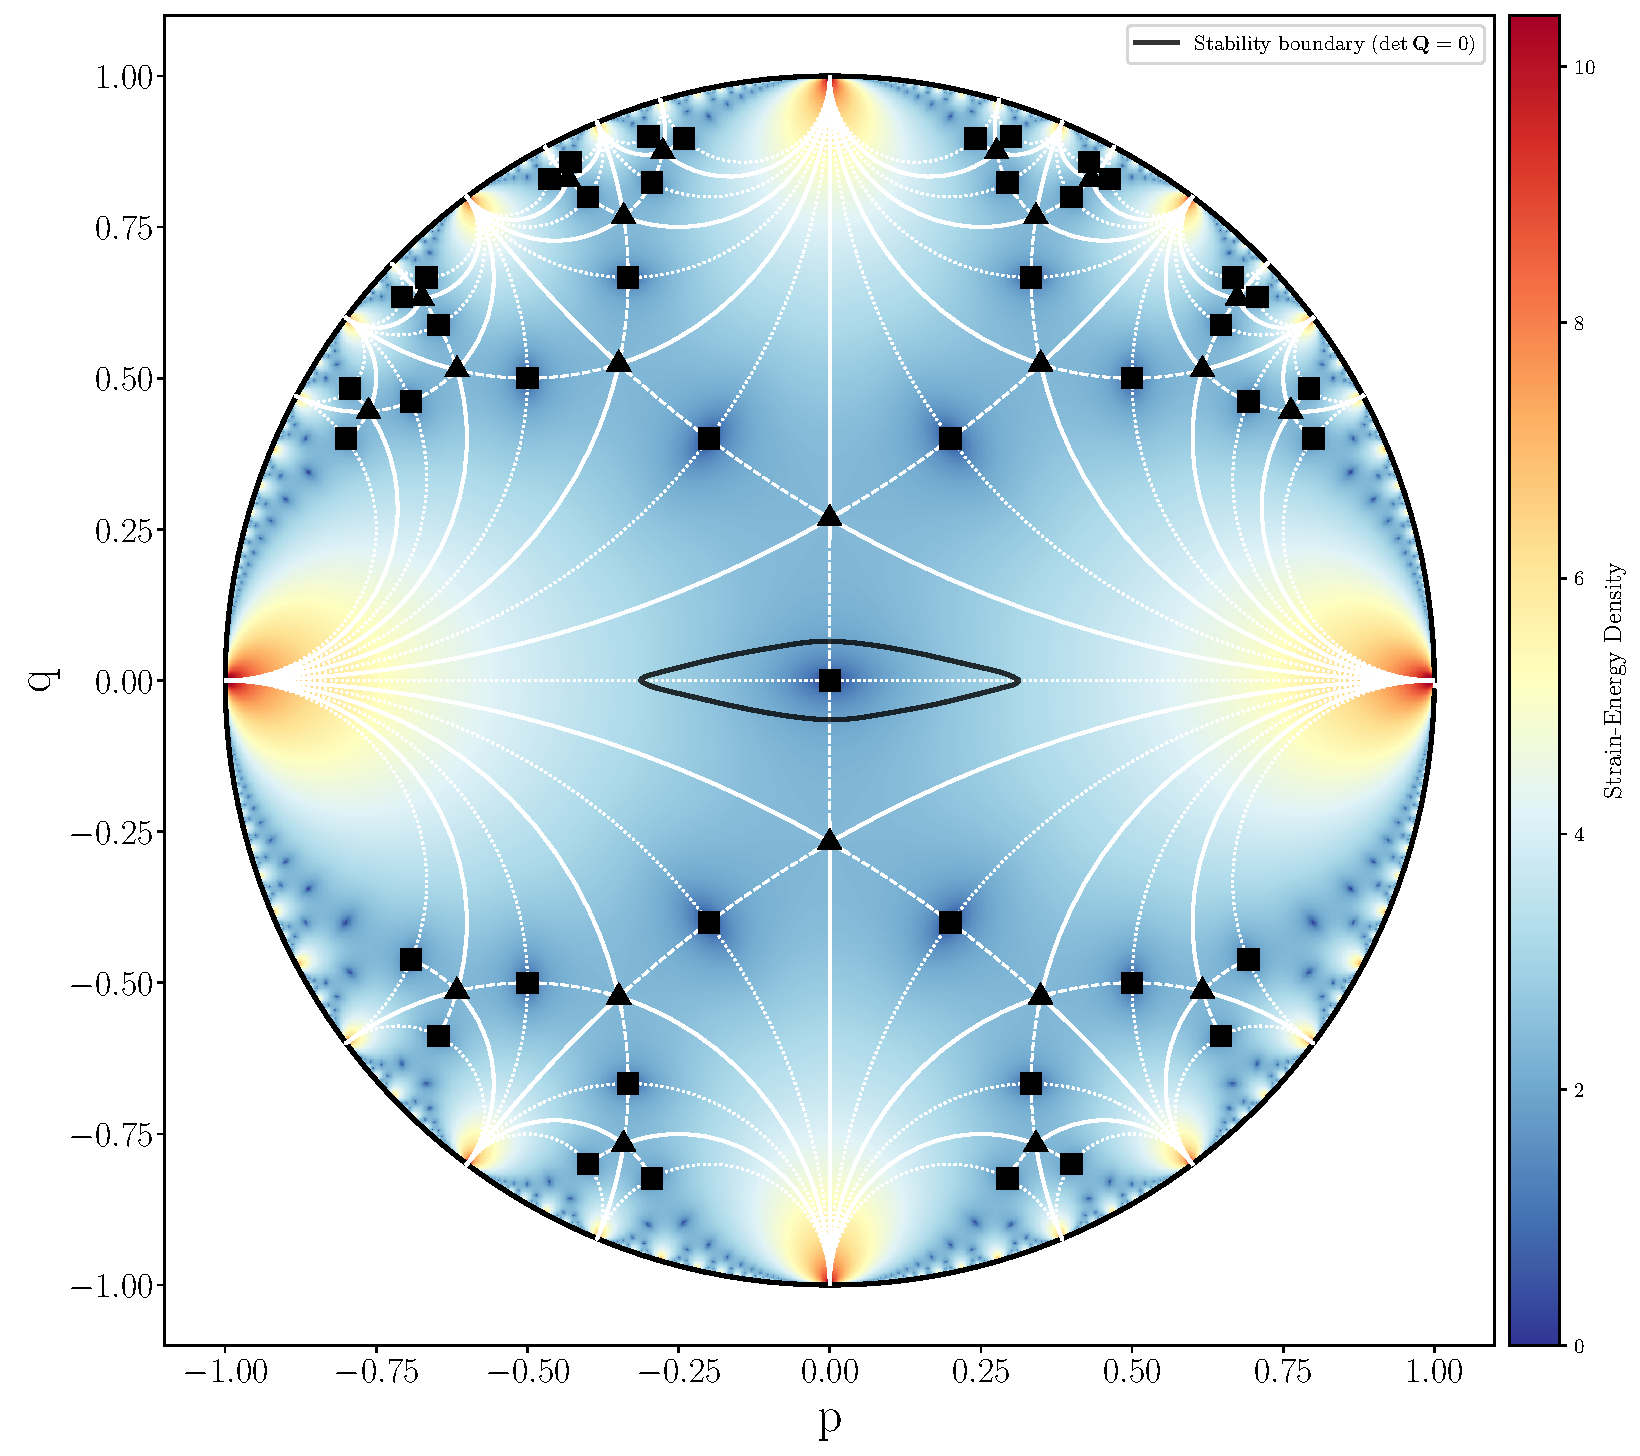
\includegraphics[scale=0.25]{./fig_sm/Fig1.pdf}
\caption{Strain-energy density  in the configurational space $C_{11}, C_{22},C_{12}$ with  $\det{\bf C}=1$  stereographically projected on  the  Poincar\'e disk.
%  $p^2 + q^2 < 1$ where 
%$p = t(C_{11} - C_{22})/2$, 
%$q = tC_{12}$, 
%and  $t = 2/(2 + C_{11} + C_{22})$.
 Thin white lines represent  the $GL(2,\mathbb{Z})$ tessellation of the  a Poincar\'e disk  into equivalent periodicity domains. Colors represent energy levels. Elastic stability boundary given by ~\eqref{detQ} is  shown by the thick black contour surrounding  the reference state.  Small black squares and triangles correspond to equivalent square and triangular lattices, respectively.
}
\label{01}
\end{figure}



\paragraph{Elastic energy density.} While the single-period Landau potential $\phi_\mathscr{D}(\tilde{\bf C})$ can be   constructed using the classical Cauchy-Born approach, see for instance   \cite{Baggio2023-qu, Baggio2023},  in this paper we used, for simplicity, the phenomenological expression proposed in \cite{Conti2004-sv}. Specifically, the  elastic energy density is represented as a sum of two terms:
 \begin{equation}
\phi(\tilde{\bf C}) = \phi_0 \left(\frac{\tilde{\bf C}}{(\det {\tilde{\bf C}})^{1/2}} \right) + \phi_v(\det \tilde{\bf C}), 
\end{equation}
where $\phi_0 $ accounts for contributions due to   shear   while $\phi_v$ penalizes    volumetric deformations. The $ GL(2,\mathbb{Z})$ invariant shear  term is chosen in the form  a sixth-order polynomial  which is the minimal requirement  ensuring   stress continuity over the whole configurational space  \cite{Parry1998,Conti2004-sv}. It depends on a single parameter $\beta$ allowing one to associate   ground state either with square or triangular (hexagonal) lattice 
 \begin{equation}\label{enerC}
 \phi_0 \left( \frac{\tilde{\bf C}}{(\det {\tilde{\bf C}})^{1/2}} \right) = \beta\psi_1\left( \frac{\tilde{\bf C}}{(\det {\tilde{\bf C}})^{1/2}} \right) + \psi_2\left( \frac{\tilde{\bf C}}{(\det {\tilde{\bf C}})^{1/2}} \right). 
 \end{equation}
The requirement of stress continuity across the whole periodic energy landscape specifies the functions $\psi_1$ and $ \psi_2$ 
\begin{align}
\psi_1 &= I_1^4 I_2 - \frac{41}{99} I_2^3 + \frac{7}{66} I_1 I_2 I_3 + \frac{1}{1056}I_3^2, \\
\psi_2 &= \frac{4}{11} I_2^3 + I_1^3 I_3 - \frac{8}{11} I_1 I_2 I_3 + \frac{17}{528} I_3^2.
\end{align}
where  we used  the known hexagonal invariants of the metric tensor 
\begin{align}
I_1 &= \frac{1}{3}(\tilde{C}_{11} + \tilde{C}_{22} - \tilde{C}_{12}), \\
I_2 &= \frac{1}{4}(\tilde{C}_{11} - \tilde{C}_{22})^2 \nonumber\\
    &\quad + \frac{1}{12}(\tilde{C}_{11} + \tilde{C}_{22} - 4\tilde{C}_{12})^2, \\
I_3 &= (\tilde{C}_{11} - \tilde{C}_{22})^2(\tilde{C}_{11} + \tilde{C}_{22} - 4\tilde{C}_{12}) \nonumber\\
    &\quad - \frac{1}{9}(\tilde{C}_{11} + \tilde{C}_{22} - 4\tilde{C}_{12})^3.
\end{align}
We select   $\beta = -1/4$ to   ensure  that global energy minimizers correspond to square lattices. 
 The volumetric part of the energy density, which primarily influences the fine structure of the dislocation cores   and also controls the formation of voids, is assumed to be of a generic form preventing infinite compression
 % \begin{equation}
$ \phi_v(s) = \mu(s - \log(s)). $
% \end{equation}
  To keep in our numerical experiments the strain field close to the surface $\det{\bf C} = 1$, we adopted   a sufficiently high value of the bulk modulus,  $\mu = 5$. 

 
The isochoric part of the  energy landscape is illustrated in Fig. 2 of the main paper. Here we also show the same Landau-type potential in Fig. \ref{01}, but now in the level set representation. Dark blue regions  correspond to the equivalent square energy wells. Red domains  show effectively inaccessible regions where the energy is very high (truncated). Relatively low energy valleys colored in yellow correspond roughly to two simple shear plastic 'mechanisms' available in square lattices. 

 

\paragraph{Internal length scale.} 
The lack of convexity of the potential is a property which  the MTM   shares with other similar Landau-type continuum theories. In the MTM  approach the necessary regularization  is  introduced by bringing  into the model   an internal  scale  $h$ through  explicit spatial discretization.    If $L$ is the linear size of the macroscopic domain and $N^2$ is the number  of  nodes in the mesoscopic  grid, then the parameter $h=L/N$  introduces elastic finite  elements imitating mesoscopic aggregates of atomic particles and defines in this way the  cutoff beyond which the deformation is considered homogeneous (affine).  The corresponding small parameter is $\delta=h/L=1/N$. Another small parameter in the problem is  $\epsilon=a/L$ where $a$ is  the   interatomic distance and we  are interested in the  double limit:  $\epsilon \to 0$  and $\delta \to 0$ while  $\delta\gg\epsilon$. In the MTM approach  we first implicitly perform the limit $\epsilon \to 0$ and recover in this way  the  continuum  constitutive response    using  the  Cauchy-Born rule. Then instead of performing the  classical  $\delta \to 0$ and obtaining the conventional scale-free continuum theory,  we preserve in the theory a small but finite value of the parameter $\delta$. In this way we effectively account for finite size effects. In particular, the size of the dislocation cores is overestimated while the number of dislocations is underestimated. However, the resulting approach  preserves the basic nature of  both long-range and short-range interactions of dislocations  at least when they are  away from the boundaries. For instance, the  blown up dislocations   will still  nucleate and self-lock adequately. 

In our numerical code we used dimensionless parameters $\tilde h=h/b=1$ and $\tilde L=L/b=1/N$, where the $b$ is the size of the mesoscopic particle. For the choice of the   scale $b$ it is natural to require  that  the  Cauchy-Born   energy density   computed for a lattice fragment with  scale $b$   exhibits a high level of  periodicity within  the  range of strains reached in a particular  numerical experiment.  We have checked that in our case the assumption that $b \sim 10 a$ is sufficient. 

 
 \paragraph{Numerical method.}
 
  Numerical implementation of the MTM approach reduces to solving an elastic finite element problem.  The goal is to follow the displacements of the   network of discrete nodes  labeled by integer-valued coordinates $I =1,..., N^2$. 
  
  Specifically, we assume that each  of the  elements  is a deformable triangle and  employ the standard  linear  3-node elements  \cite{Irons1966,Bramble1970-oq}. The displacement field  inside each of  the elements,  represented  in   dimensionless form,  can be written in the form
%\begin{equation}
 ${\bf u} ({\bf z}) = \sum_{a } \mathcal{N} ^a({\bf z};h) {\bf u}^a,$
 %\end{equation}
 where ${\mathcal N}^a(\bf z;h)$ are   compactly supported  linear shape functions,  ${\bf u}^a$ are the are the
nodal displacements and summation is assumed over repeated indexes; the interpolation functions for each element are defined in terms of a local  dimensionless coordinate system. The mesoscopic deformation gradient is then 
 %\begin{equation}
 ${\bf F}({\bf z}; h) =\mathbb{I}+ {\bf u} ^a\otimes\nabla\mathcal{N} ^a({\bf z};h).$ 
% \end{equation}

 In terms of macroscopic reference coordinates,  the elastic energy inside each element can be  computed using the simplest   quadrature scheme 
%\begin{equation}
$w ({\bf x}; h)=\frac{1}{2}  \phi({\bf F} ({\bf x}; h)) J({\bf x},h),$
%\end{equation}
where $J$ is the Jacobian of the transformation from local ($\bf z$)   to  global ($\bf x$) coordinate system. Note that in view of our assumptions the  energy of a  deformed triangular element depends on  three parameters:  the deformed lengths  of the bonds   and   the deformed value of the angle between them. 
 


Finding  a solution of an elastic problem implies  local minimization of the energy 
%\begin{equation}
$W=\int_{\Omega}w({\bf x}; h)  d\mathbf{x}, $
%\end{equation}
which is prescribed on a triangulated  domain \(\Omega\).   The conditions of mechanical equilibrium take the form 
 $\nabla\cdot\mathbf{P}=0$ where we introduced  the first Piola-Kirchhoff stress tensor 
%\begin{equation}
%$\mathbf{P}= 2\mathbf{F} \mathbf{m} \frac{\partial w }{\partial \tilde{\bf C}}\mathbf{m}^T,$
%\end{equation}
 $$\mathbf{P}= 2\mathbf{F} \mathbf{m}{\bf \Sigma}\mathbf{m}^T,$$ with  $${\bf \Sigma} = \begin{bmatrix}
\frac{\partial w}{\partial \tilde{C}{11}} & \frac{1}{2}\frac{\partial w}{\partial \tilde{C}{12}} \\
\frac{1}{2}\frac{\partial w}{\partial \tilde{C}{12}} & \frac{\partial w}{\partial \tilde{C}{22}}
\end{bmatrix}.$$ In the finite element representation these  equations reduce to 
%\begin{equation}
$$\frac{\partial W}{\partial \mathbf{u}^{a}}=\int_{\Omega} \mathbf{P}(\mathbf{x};h) \nabla \mathcal{N}^{a} (\mathbf{x};h) d\mathbf{x} = 0.$$ 
%\end{equation} 




The ensuing nonlinear equilibrium problem is solved numerically using the L-BFGS algorithm~\cite{Bochkanov2013-lk}, which constructs a positive definite approximation to the Hessian, enabling quasi-Newton steps that progressively reduce the total energy. Iterations continue until the energy change per iteration falls below a prescribed tolerance. At each iteration, starting from an approximate solution ${\bf w}^a$, we compute a displacement correction $\text{d}{\bf w}^a={\bf u}^a-{\bf w}^a$ by solving the linearized equilibrium equations via LU factorization~\cite{Sanderson2016-ht,Fishman2022-nj}:
$$K^{ab}_{ij}dw_j^b+R_i^a =0,$$
where$$K^{ab}_{ij}= A_{ipjq}({\bf F}) \frac{\partial {\mathcal N}^a}{\partial x_p}\frac{\partial {\mathcal N}^b}{\partial x_q} $$ is the global stiffness matrix and $$R^a_i= P_{ip}( {\bf F}) \frac{\partial {\mathcal N}^a}{\partial x_p},$$is the residual force vector 
with summation implied over repeated indices. Note that  we introduced  the tensor of tangential elastic moduli
$$A_{iajb}= \frac{\partial^2\phi_\mathscr{D}{({\bf \tilde C} )}}{\partial F_{ia}\partial F_{jb}}.$$ which  can be used construct the Eulerian acoustic tensor
$${Q}_{ij}=F_{la} F_{mb} A_{iajb} n_l n_m,$$
where $\bf n$ is an arbitrary unit vector. The Legendre-Hadamard  condition  which marks the threshold of elastic instability in continuum theory can be  then written in the form
\begin{equation} \label{detQ}
\det (\boldsymbol{{Q}})=0.
\end{equation}
The corresponding  stability boundary is referred to in the main paper and it is illustrated for the  chosen elastic energy landscape  in Fig.~\ref{01}.


% The ensuing mathematical  problem is solved numerically using the L-BFGS algorithm~\cite{Bochkanov2013-lk} which builds a positive definite linear approximation allowing one to make a quasi-Newton step lowering the total energy.   \textcolor{blue}{The   iterations continue until the change in total energy per iteration becomes sufficiently small.} More specifically,  an approximate solution is   used as an initial guess  ${\bf w}^a$ to solve, using LU factorization~\cite{Sanderson2016-ht,itensor},  the linear  equations for the correction  $\text{d}{\bf w}^a={\bf u}^a-{\bf w}^a$  which are of the form 
%% around   an initial guess for the displacement field  ${\bf u}^a={\bf w}^a +  \text{d}{\bf w}^a.$ 
%  % The corresponding  system of linear equations  
%   %\begin{equation}
% $K^{ab}_{ij}dw_j^b+R_i^a =0,$
% %\end{equation}
%  where 
%%\begin{equation}
%$K^{ab}_{ij}= A_{ipjq}({\bf F}) \frac{\partial {\mathcal N}^a}{\partial x_p}\frac{\partial {\mathcal N}^b}{\partial x_q}$ and $ R^a_i= P_{ip}( {\bf F}) \frac{\partial {\mathcal N}^a}{\partial x_p}.$
%%\end{equation}
%%Note that   we used the Eulerian $i,j=1,2$ and the Lagrangian $K,L =1,2$ indexes and assumed summation over repeated indexes.  
%Here we  also defined   the tensor of tangential elastic moduli
% %\begin{equation}
%$ A_{iajb}= \frac{\partial^2\phi_D{({\bf \tilde C} )}}{\partial F_{ia}\partial F_{jb}}.$
%%\end{equation}
%Note that using the Eulerian acoustic tensor  
% %\begin{equation}\label{Q}
%$ {Q}_{ij}=F_{la} F_{mb} A_{iajb} n_l n_m,$
% %\end{equation}
%  where $\bf n$ is a  unit vector, we can obtain   the Legendre-Hadamard threshold of   elastic instability 
%  \begin{equation} \label{detQ}
% \det (\boldsymbol{{Q}})=0, 
%  \end{equation}  
% as used in the main paper and illustrated for our chosen elastic energy 
%density in Fig. \ref{01}.
%  
%  of the corresponding continuum body  in the form \cite{Ogden1997-rf,Grabovsky2014-fb}
  
%This condition is illustrated for the chosen energy density in Fig. \ref{01}.  
% 


%\subsection{Periodic Boundary Conditions with Macroscopic Deformation}

 \paragraph{Implementation of the loading conditions. } To simulate an effectively infinite crystal under controlled  macroscopic affine deformation, we use the method of domain replication. Starting from the computational domain $\Omega_0$ with dimensions $L_x \times L_y$,
 % is replicated in all spatial directions to create a periodic array of domains. 
we generate a periodic lattice of domains using  translation vectors  
 $\mathbf{t}_n = \begin{pmatrix} n_x L_x \\ n_y L_y \end{pmatrix},$ where  $\mathbf{n} = (n_x, n_y) \in \{-1, 0, 1\}^2.$ 
%where $\mathbf{n}$ represents the integer lattice coordinates.
% For the 9-domain implementation, we consider all translation vectors within the immediate neighborhood of the central domain. 
 Let $\bar{\bf F}(\alpha )$ denote the macroscopic deformation gradient tensor at  the parameter value  $\alpha$. Under such affine deformation, the position of   replicated domains relative to the central domain $\Omega_0$ is given by:
 $\mathbf{R}_n = \bar{\bf F}(\alpha ) \cdot \mathbf{t}_n,$ 
where $\mathbf{R}_n$ represents the displacement vector of the origin of the domain associated with $\mathbf{t}_n$. 
Then, for a node located at position $\mathbf{x}_i$ in the central domain $\Omega_0$, its periodic image, associated with the  translation vector $\mathbf{t}_n$, is at:
 $\mathbf{x}_i^{(n)} = \mathbf{x}_i + \mathbf{R}_n = \mathbf{x}_i + \bar{\bf F}(\alpha ) \cdot \mathbf{t}_n.$ 
Such correspondence ensures that the macroscopic deformation gradient $\bar{\bf F}(\alpha )$ is consistently applied across all periodic images of $\Omega_0$. After establishing the positions of all nodes across the nine domains (original domain $\Omega_0$ and its eight periodic images), we perform a Delaunay triangulation on the complete set of particles:
 $\mathcal{P} = \{\mathbf{x}_i : i \in \mathcal{I}_0\} \cup \{\mathbf{x}_i^{(n)} : i \in \mathcal{I}_0, n \neq \mathbf{0}\},$ 
where $\mathcal{I}_0$ denotes the set of particle indices in the original domain and $\mathbf{0} = (0,0)$ corresponds to the null translation vector.  Using the obtained global  triangulation $\mathcal{T}$, we select  the  triangles that have at least one vertex belonging to the original domain $\Omega_0$. 
\begin{figure}[h!]
\centering
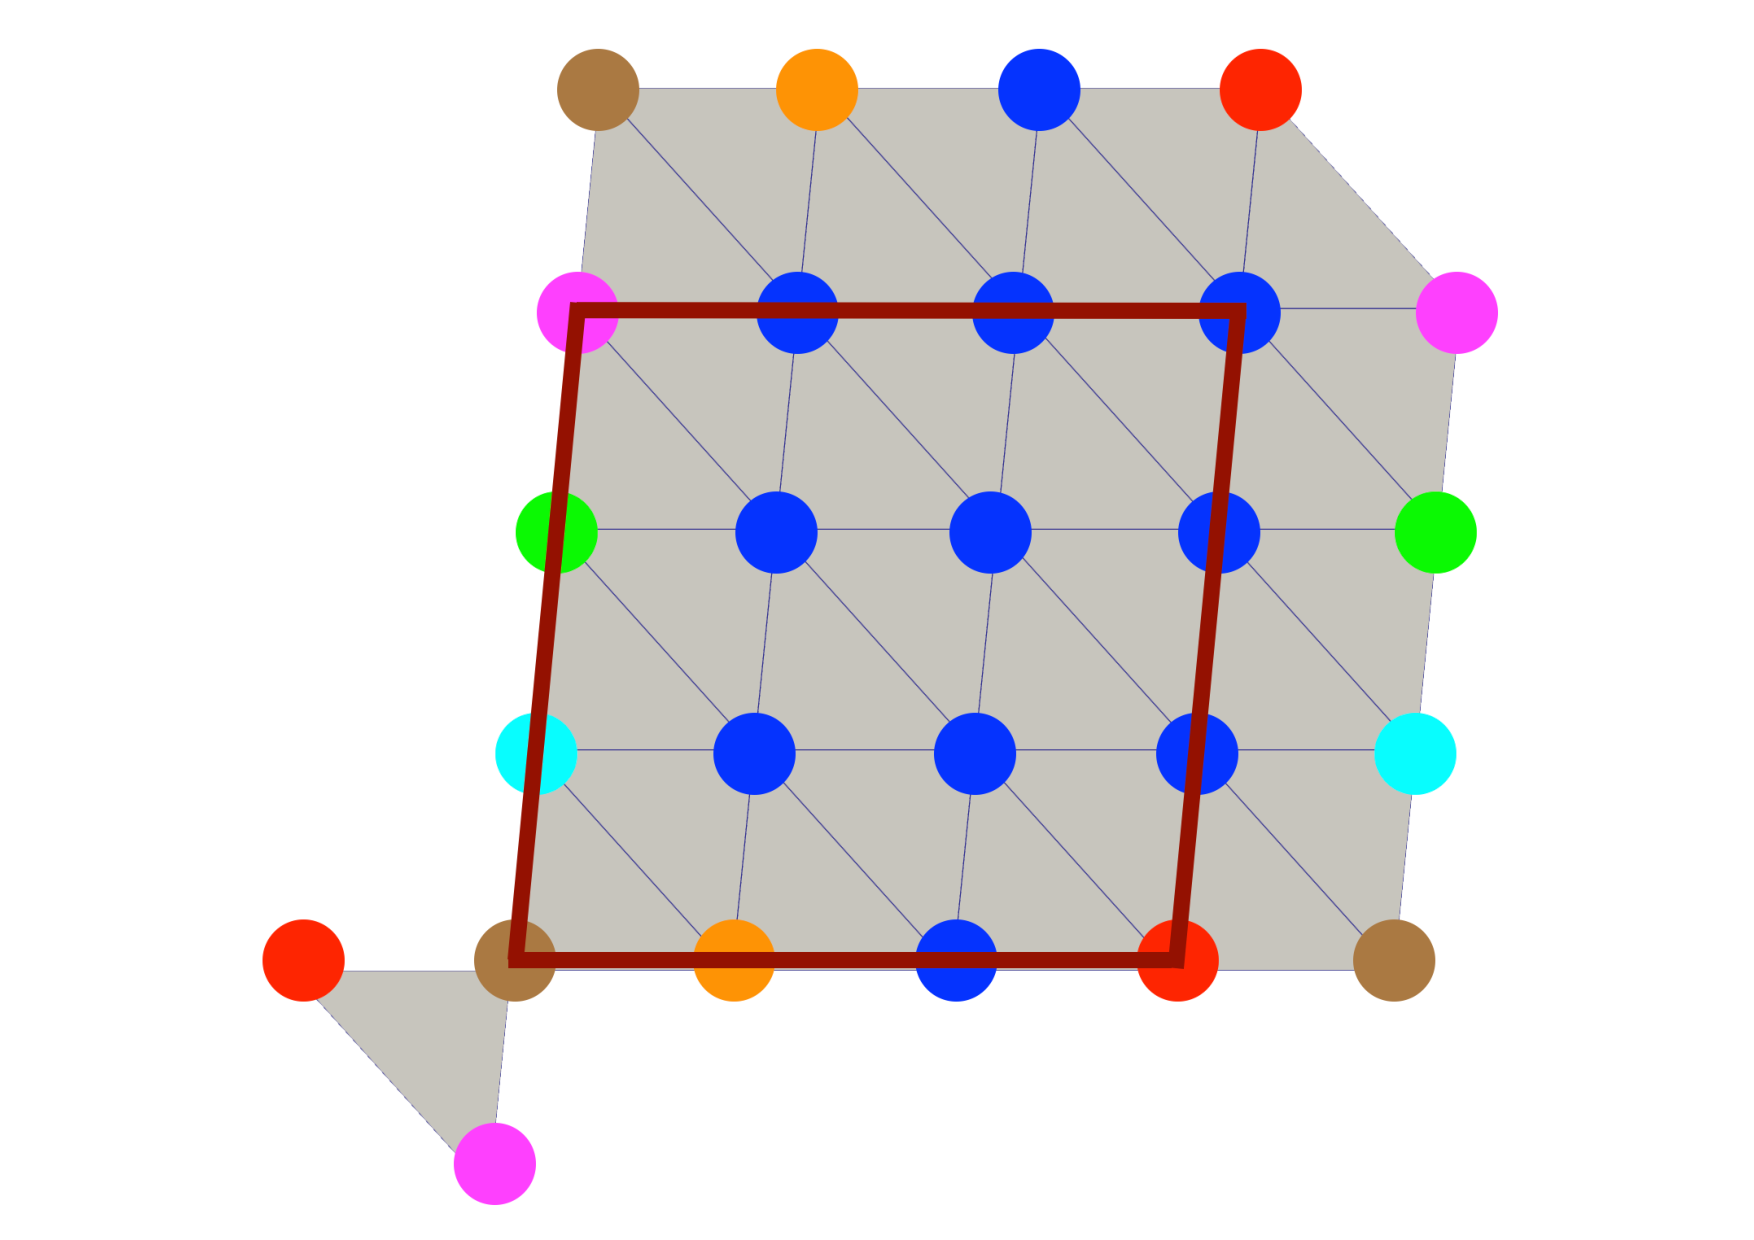
\includegraphics[scale=0.15]{./fig_sm/Fig2.pdf}
\caption{ The periodicity unit of the computational mesh $\mathcal{T}_{\text{ch}}$  obtained by  periodic Delaunay triangulation. The central computational domain $\Omega_0$ is limited by the brown box. Only triangles with at least one vertex in $\Omega_0$ are selected for the mesh (shown by the thin lines), ensuring proper connectivity across periodic boundaries while avoiding redundant counting of triangles.
}\label{sm:fig2}
\end{figure}


Note that  since triangles near periodic boundaries may be counted multiple times through different domain images, we need to ensure  uniqueness by mapping all vertex indices to their representatives in $\Omega_0$ and using the sorted tuple of these representatives as a canonical identifier. 

Specifically, a triangle is included in the chosen mesh $\mathcal{T}_{\text{ch}}$ only upon its first encounter, ensuring that each physical triangle is counted exactly once. The ensuing periodicity unit of the computational mesh $\mathcal{T}_{\text{ch}}$  is illustrated in Fig.~\ref{sm:fig2}, where we show the central domain $\Omega_0$ (limited by the brown box) together with   triangles associated with the nodes  constituting this domain.  Such  selection  procedure ensures that:
(i) Each triangle in the computational mesh is counted exactly once, eliminating redundancy from the periodic extension; (ii)
 All triangles connected to the original domain are included, maintaining proper connectivity across periodic boundaries;
(iii) The triangulation naturally incorporates the macroscopic deformation through the deformed positions of the periodic images.

 The selected set of triangles $\mathcal{T}_{\text{ch}}$ was used as the computational mesh in the MTM based numerical experiments  ensuring both, compatibility  with   the periodic boundary conditions and  consistency with the applied macroscopic deformation gradient $\bar{\bf F}(\alpha )$.  

%\begin{figure}[h!]
%\centering
%\includegraphics[scale=0.25]{Figures_ordered_old/fig_3_SM.pdf}
%\caption{Probability distributions of stress drop avalanches ($S=\Delta \sigma_{xy}A$) for the (blue) pre-yield and (red) post-yield regimes with different exponents.}
%\label{sm:fig3}
%\end{figure}
% \textcolor{blue}{\paragraph{Stress drop distributions and non-monotonic scaling}
%We define avalanches from the stress drops as $S=A\Delta\sigma_{xy}$, where $A$ is the initial surface of the crystal. The probability distributions $P(S)$ for the pre- and post-yield regimes are shown in Fig. \ref{sm:fig3}. In the pre-yield regime, we find a power-law exponent $\epsilon \approx 1.1$, while in the post-yield regime, the distribution exhibits a steeper decay with $\epsilon \approx 1.28$. This shift in exponents is coupled to a non-monotonic scaling relationship between the mean stress drop and dissipated energy, $\langle S \rangle \sim E^{\eta}$, observed across both stages of deformation. \textit{Pre-yield Multi-scale Scaling.} In the pre-yield regime, the scaling $\eta$ exhibits a characteristic crossover from $\eta \approx 0.26$ for small events to $\eta \approx 0.71$ for larger avalanches. The low initial value represents a "mechanically silent" stage where localized dislocation rearrangements dissipate energy without significant macroscopic stress relief. As event size increases, the strengthening of the coupling to $\eta \approx 0.71$ indicates the onset of more extended dislocation activity. In this regime, the stress exponent ($\epsilon \approx 1.1$) remains closely matched to the energy exponent, reflecting a scale-free state where the avalanche cutoff may be governed by the micro-structural state as  dislocation density rather than proximity to a critical stress. \textit{Post-yield Non-monotonicity and Exponent Divergence.} In the post-yield regime, the scaling $\eta$ remains non-monotonic but shifts to higher efficiency, transitioning from $\eta \approx 0.13$ for small-scale restructuring to $\eta \approx 0.81$ for large, collective avalanches. This transition marks the emergence of system-spanning shear bands.} 
% 
%\begin{figure}[!hbt]
%    \centering
%    \includegraphics[scale=0.145]{Figures_ordered/fig_4_SM_h.pdf}
%    \caption{Scaling relationship between stress and energy drops in pre-and post-yield regimes.} 
%
%    \label{sm:fig4}
%\end{figure}

%\bibliography{./formatted.bib}
%merlin.mbs apsrev4-1.bst 2010-07-25 4.21a (PWD, AO, DPC) hacked
%Control: key (0)
%Control: author (8) initials jnrlst
%Control: editor formatted (1) identically to author
%Control: production of article title (-1) disabled
%Control: page (0) single
%Control: year (1) truncated
%Control: production of eprint (0) enabled

\paragraph{Finite Size Scaling and Data Collapse.}
To determine the power-law exponent and the finite-size scaling exponent (often interpreted as the fractal dimension of the avalanches), we employ a robust data-collapse optimization procedure. Near the critical point, the probability distribution $P(s;L)$ of avalanche sizes $s$, which can represent either the dissipated energy $\Delta W$ or the macroscopic stress drop $S$ (defined as the drop in the Cauchy stress tensor component $\sigma_{xy}$ multiplied by the current surface area $A$, yielding $S = A \Delta\sigma_{xy}$), for a system of linear size $L=Nh$ obeys the finite-size scaling (FSS) ansatz:
\begin{equation}
  P(s; L) \;=\; s^{-x}\, \mathcal{F}\!\left(\frac{s}{L^{D_x}}\right),
\end{equation}
where $x$ represents the relevant power-law exponent ($x = \tau$ for stress drops and $x = \epsilon$ for dissipated energy), $D_x$ is the corresponding fractal dimension ($D_\epsilon$ or $D_\tau$), and $\mathcal{F}(u)$ is a universal scaling function. Rather than relying on the algebraic moment spectrum, we directly rescale the axes to collapse distributions from all system sizes onto a single master curve. We define the rescaled variables:
\begin{equation}
  \tilde{x}(s,L) \;=\; \frac{s}{L^{D_x}},
  \qquad
  \tilde{y}(s,L) \;=\; P(s;L)\cdot L^{D_x x}.
\end{equation}
The optimal parameters $(x^*, D_x^*)$ are determined by minimizing the residual spread between the rescaled curves across their common overlapping range. For a discrete set of system sizes $\{L_k\} = N_kh$, the quality of the collapse at a trial pair $(x,D_x)$ is evaluated systematically. First, we compute the discrete logarithmic data points $(u_{k,i}, v_{k,i}) = (\log_{10}\tilde{x}_{k,i}, \log_{10}\tilde{y}_{k,i})$ for each system size $L_k$.

Next, we determine the common logarithmic interval by identifying the overlapping limits $u_{\min} = \max_k[\min_i(u_{k,i})]$ and $u_{\max} = \min_k[\max_i(u_{k,i})]$. For our datasets, a robust overlap domain naturally exists near the optimal scaling exponents. We then define a uniform grid of 80 points $\{c_j\}$ spanning the interval $[u_{\min}, u_{\max}]$. To evaluate the curves on this common grid, we construct a continuous function $\hat{v}_k(u)$ for each system size using linear interpolation between the discrete points $(u_{k,i}, v_{k,i})$.

We define the valid index set $\mathcal{V}$ as the subset of grid indices $j$ such that the grid point $c_j$ lies strictly within the measured domain of all $N_L$ interpolated curves, ensuring no extrapolation is required. The quality of the collapse is quantified by computing the average variance across this valid set:
\begin{equation}
  \mathcal{Q}(x,D_x) 
  = 
  \frac{1}{|\mathcal{V}|} \sum_{j\in\mathcal{V}} \left( \frac{1}{N_L - 1} \sum_{k=1}^{N_L} \left[ \hat{v}_k(c_j) - \bar{v}(c_j) \right]^2 \right),
  \label{eq:quality}
\end{equation}
where $\bar{v}(c_j) = \frac{1}{N_L} \sum_{k=1}^{N_L} \hat{v}_k(c_j)$ is the mean value of the interpolated curves at the fixed grid point $c_j$.

Evaluating this collapse variance provides a highly sensitive measure of how well the distributions coincide. We employ a two-stage grid-search (first coarse, then fine) in the $(x, D_x)$ parameter space to locate the global minimum of the variance, $\mathcal{Q}_{\text{min}}$. The coordinates of this minimum define the optimal scaling exponents, $(x^*, D_x^*)$. 

To estimate the uncertainties of these exponents, we analyze the curvature of the $\mathcal{Q}$ landscape immediately surrounding the minimum. For each parameter, we project the variance onto a 1-D profile and fit it with a parabola. Because traditional statistical error models do not strictly apply to this data-collapse metric, we establish an operational threshold for the error: the $1$-$\sigma$ confidence interval is defined as the parameter deviation required to double the variance from its optimal value (i.e., the half-width where the fit reaches $2\mathcal{Q}_{\text{min}}$). Consequently, a sharp, narrow minimum in the variance landscape clearly demonstrates that the scaling parameters are tightly constrained by the overlapping data.

\begin{figure}[hbt!]
\centering
\begin{tabular}{cc}
(a) & (b) \\
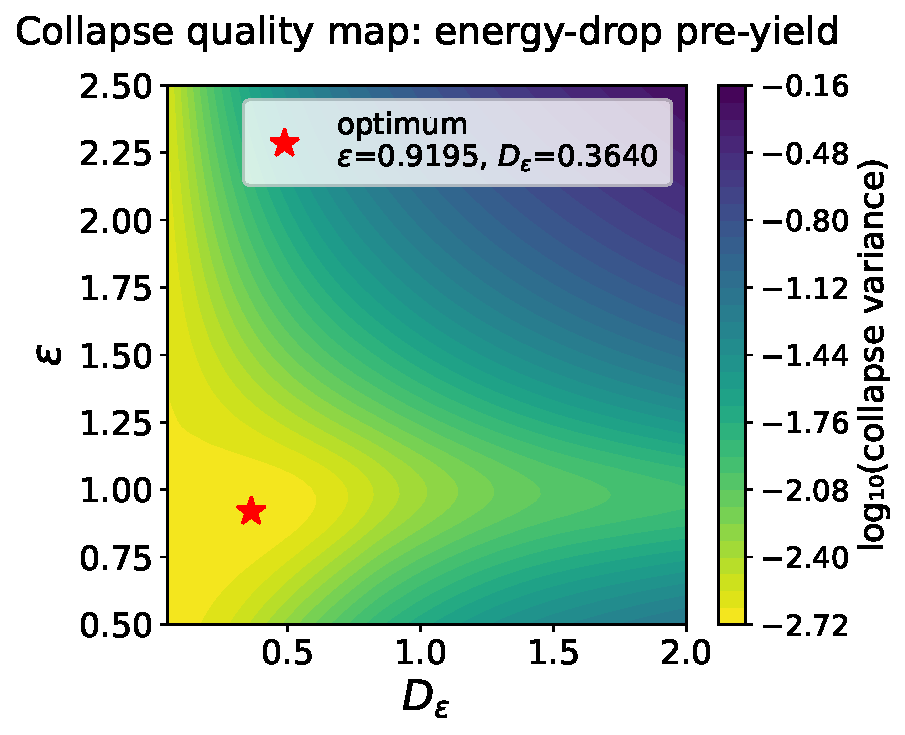
\includegraphics[width=0.21\textwidth]{./fig_sm/Fig3-a.pdf} &
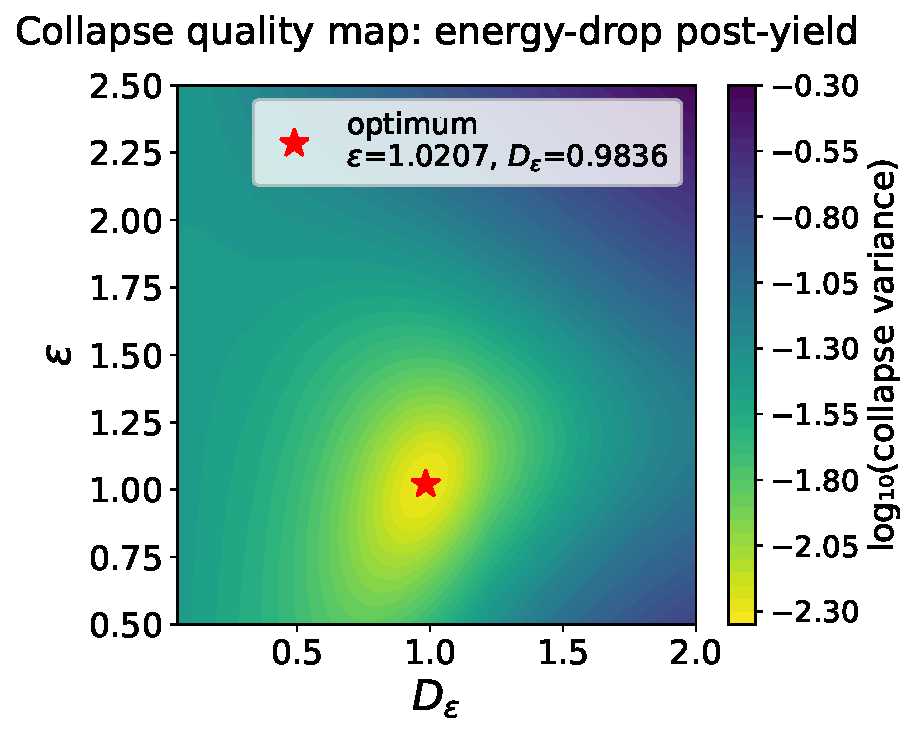
\includegraphics[width=0.21\textwidth]{./fig_sm/Fig3-b.pdf} \\
\end{tabular}
\caption{Quality metric $\mathcal{Q}$ landscapes for the pre- and post-yield data collapse optimization. (a) Quality map $\mathcal{Q}(\epsilon,D_\epsilon)$ in pre-yield, and (b)  post-yield for the dissipated energy. The deep, well-defined global minima in these variance surfaces pinpoint the optimal scaling exponents and their geometric 1-$\sigma$ uncertainties.}
\label{sm:fig_quality_maps}
\end{figure}

\begin{figure}[hbt!]
\centering
\vspace{3mm}
\begin{tabular}{cc}
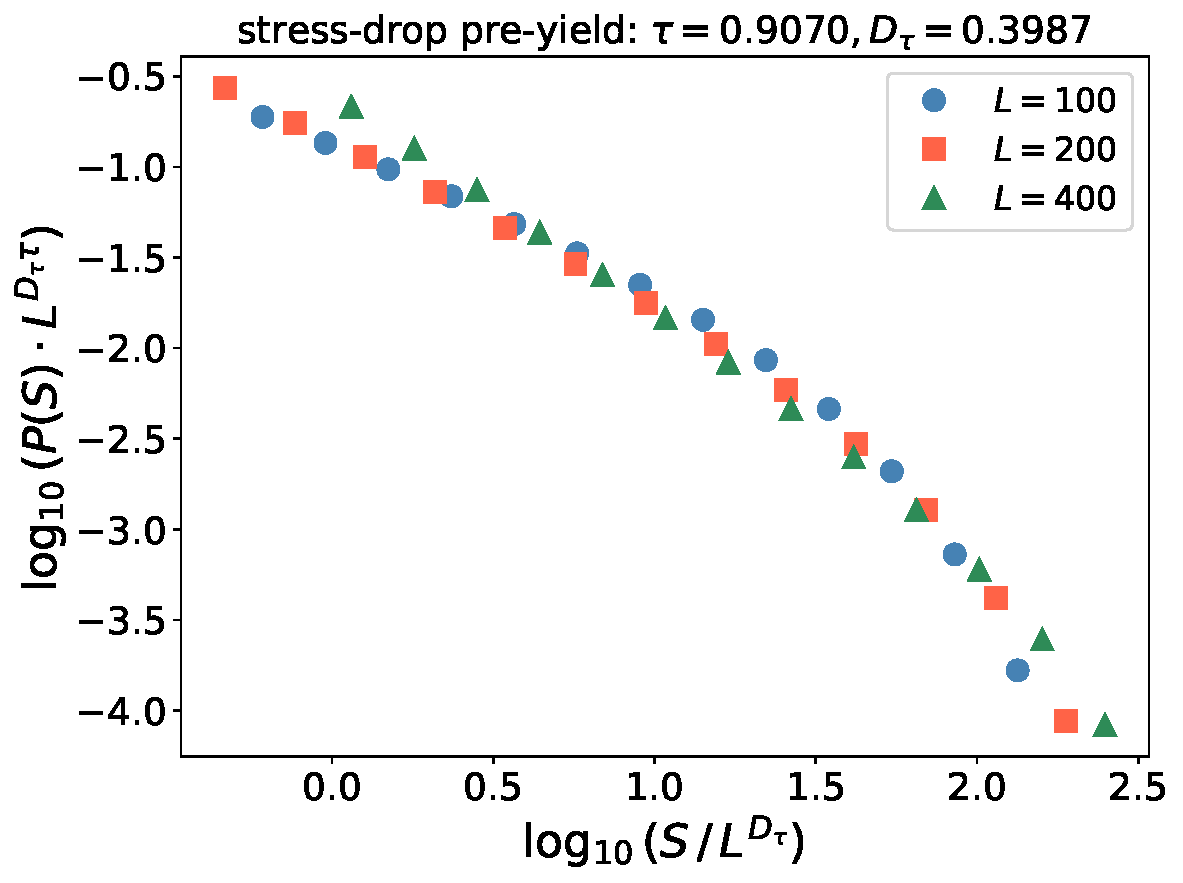
\includegraphics[width=0.2\textwidth]{./fig_sm/Fig4-a.pdf} &
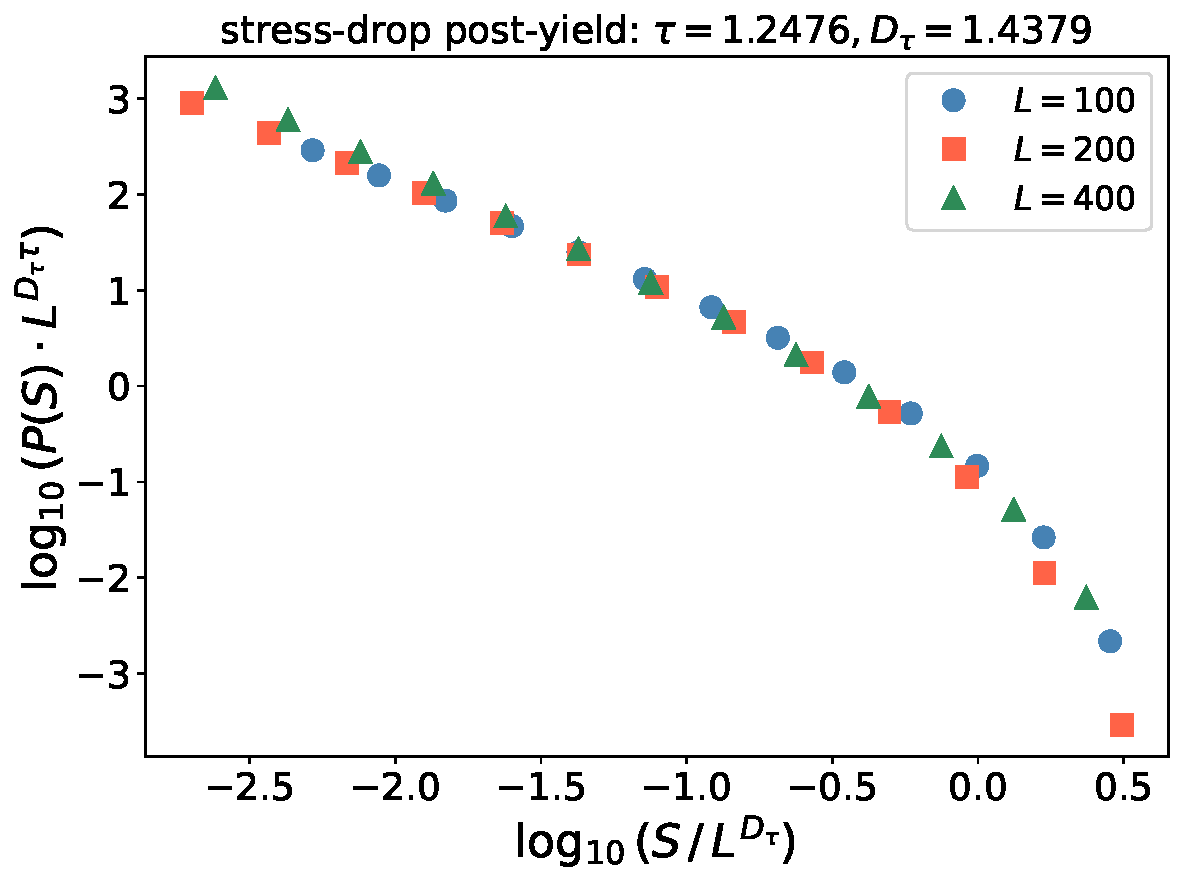
\includegraphics[width=0.2\textwidth]{./fig_sm/Fig4-b.pdf} \\
(a) Pre-yield (Stress) & (b) Post-yield (Stress) \\
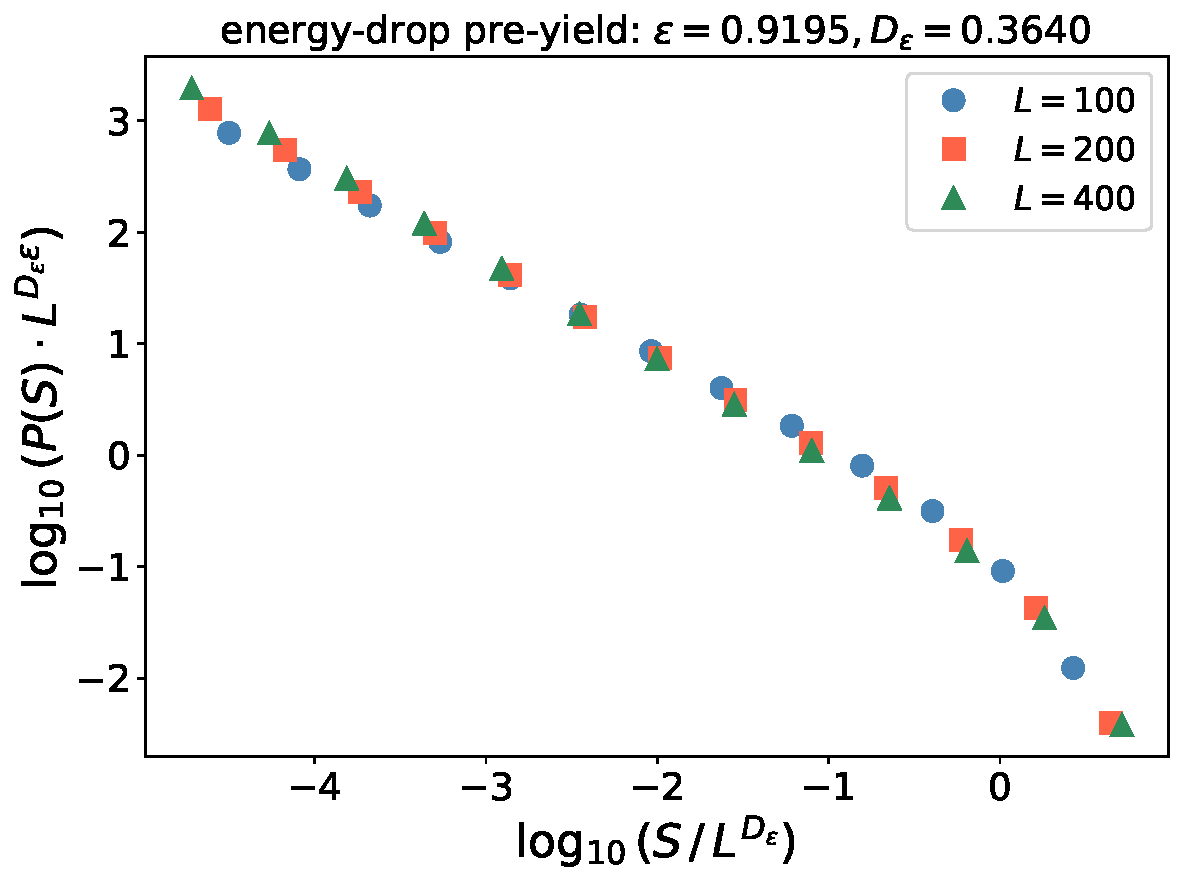
\includegraphics[width=0.2\textwidth]{./fig_sm/Fig4-c.pdf} &
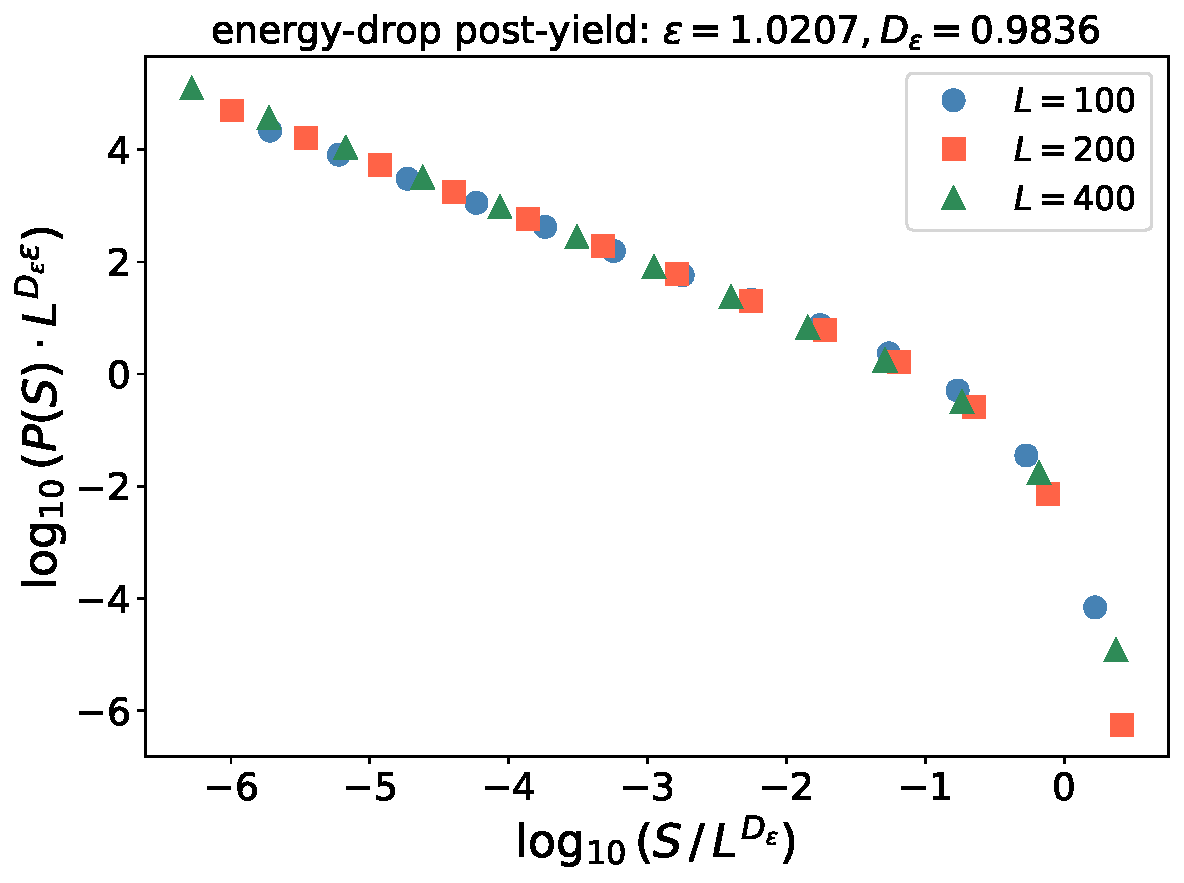
\includegraphics[width=0.2\textwidth]{./fig_sm/Fig4-d.pdf} \\
(c) Pre-yield (Energy) & (d) Post-yield (Energy) \\
\end{tabular}
\caption{Optimal data collapses of the probability distributions onto universal master curves. (a, b) Collapse of the macroscopic stress drops $S$ in the pre-yield and post-yield regimes, utilizing exponents $\tau$ and $D_\tau$. (c, d) Collapse of the dissipated energy $\Delta W$ in the pre-yield and post-yield regimes, utilizing exponents $\epsilon$ and $D_\epsilon$.}
\label{sm:fig_collapses}
\end{figure}
The variance spread landscapes and the resulting optimal data collapses are presented in Fig.~\ref{sm:fig_quality_maps} and Fig.~\ref{sm:fig_collapses}. As can be seen directly from the plots in Fig.~\ref{sm:fig_collapses}, the scaled probability distributions for different system sizes $L=Nh$ fall remarkably well onto a single universal master curve in both the pre-yield and post-yield regimes. This excellent visual overlap, spanning several decades in both probability and avalanche size, serves as strong empirical validation of the finite-size scaling ansatz and confirms the reliability of the extracted exponents. 

Crucially, the relationship between the extracted exponents for stress drops ($\tau$) and dissipated energy ($\epsilon$) reflects fundamental changes in the mechanical coupling of the active regions. In the pre-yield regime, the power-law exponents for stress and energy are remarkably similar ($\tau \approx \epsilon$). This parity suggests that the dissipated energy and the stress drop are roughly linearly proportional ($\Delta W \sim S$). Such linear scaling mechanically implies a highly constrained regime of dislocation motion—where localized interactions, such as the formation of junctions or the interference between different active gliding planes, create strong local hardening that prematurely arrests the avalanche event. Conversely, in the mature flowing post-yield regime, the measured exponents are distinctly different. In this fully plastic state, deformation is dominated by the system-spanning motion of grain boundaries sliding across the domain completely unhindered by local structural constraints, driving the dissipated energy to scale quadratically with the corresponding stress drop ($\Delta W \sim S^2$). If the macroscopic stress probability scales as $P(S) \sim S^{-\tau}$ and $\Delta W \sim S^\gamma$, probability conservation $P(\Delta W)\mathrm{d}\Delta W = P(S)\mathrm{d}S$ dictates that the energy exponent must follow $\epsilon = (\tau - 1 + \gamma)/\gamma$ (assuming basic geometric scaling relations). The phenomenological transition from linear $\gamma=1$ (pre-yield, $\epsilon = \tau$) to quadratic $\gamma=2$ (post-yield, $\epsilon = (\tau+1)/2$) naturally accounts for the physical separation of the FSS exponents observed in our data. For instance, using our measured post-yield value $\tau \approx 1.2$, the theoretical energy exponent is $\epsilon \approx 1.10$. This predicted value is in reasonable agreement with our empirically measured scaling of $\epsilon \approx 1.02$. The minor discrepancy can be directly attributed to the fact that the elastic energy density in our model is not purely quadratic in strains, but contains higher-order cubic terms that naturally perturb this idealized scaling relation. Furthermore, the uncertainties in these parameter estimations can be quite large ($\sim \pm 0.2$), and even larger simulation domains may be needed in the future to fully resolve the exact asymptotic scaling limits.

Furthermore, the extracted fractal dimensions ($D_\epsilon$ and $D_\tau$) characterize the complex geometrical morphology of the actively deforming regions. Focusing specifically on the dissipated energy avalanches, we find a stark contrast in the measured fractal dimensions between the two deformation stages. In the early pre-yield phase, the energy avalanches yield a low fractal dimension of $D_\tau \approx 0.36$, characterizing the highly localized, spatially scattered, microscopic isolated rearrangements, see Fig.~\ref{sm:fig_plastified}(a). Conversely, in the mature post-yield regime, the measured fractal dimension surges to $D_\tau \approx 0.98$. This value approaching unity is fundamentally consistent with the emergence of 1D-like system-spanning shear bands. These macroscopic bands exhibit a highly correlated, anisotropic spatial structure (fractality) as deformation localizes, naturally reflecting the cooperative, extended nature of the individual yielding events dominating the mature flowing stage, where typical avalanches include the motion of grain boundaries whose lengths are comparable to linear system (see Fig.~\ref{sm:fig_plastified}(b)).

\begin{figure}[]
\centering
\begin{tabular}{cc}
(a) Pre-yield avalanche & (b) Post-yield avalanche \\
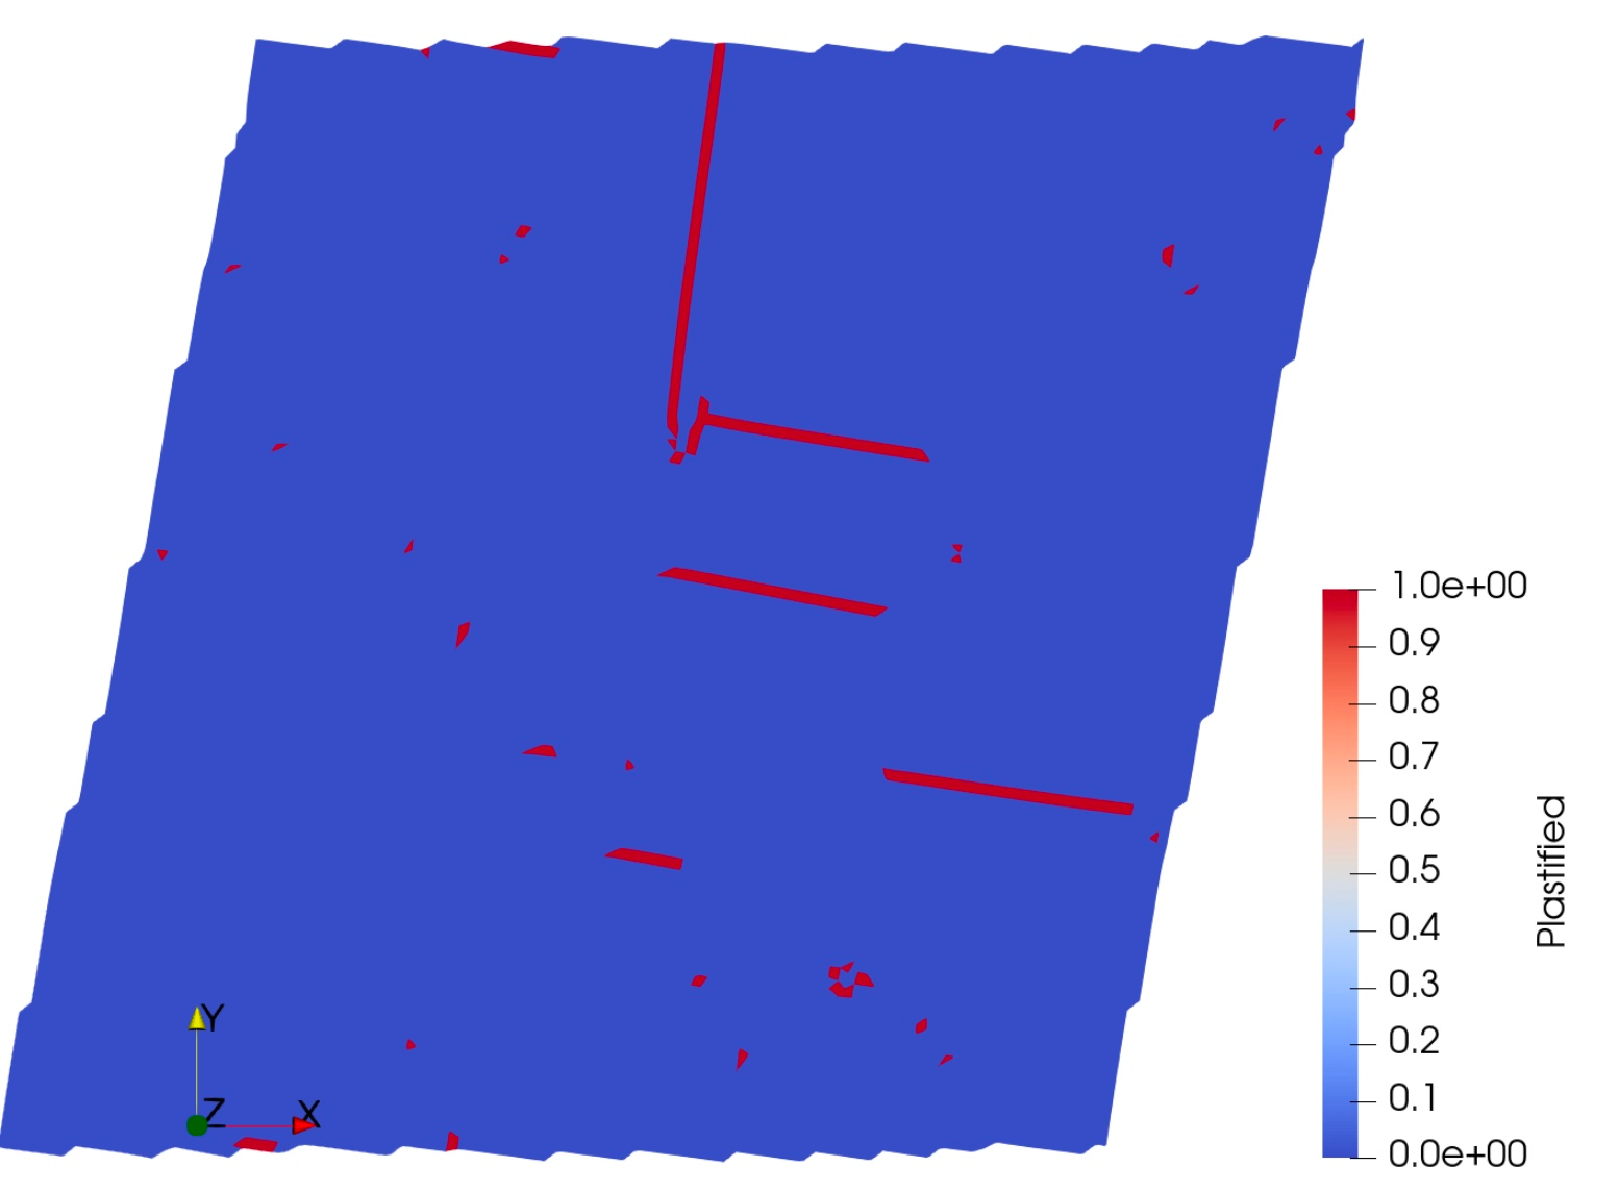
\includegraphics[scale=0.14]{./fig_sm/Fig5-a.pdf} &
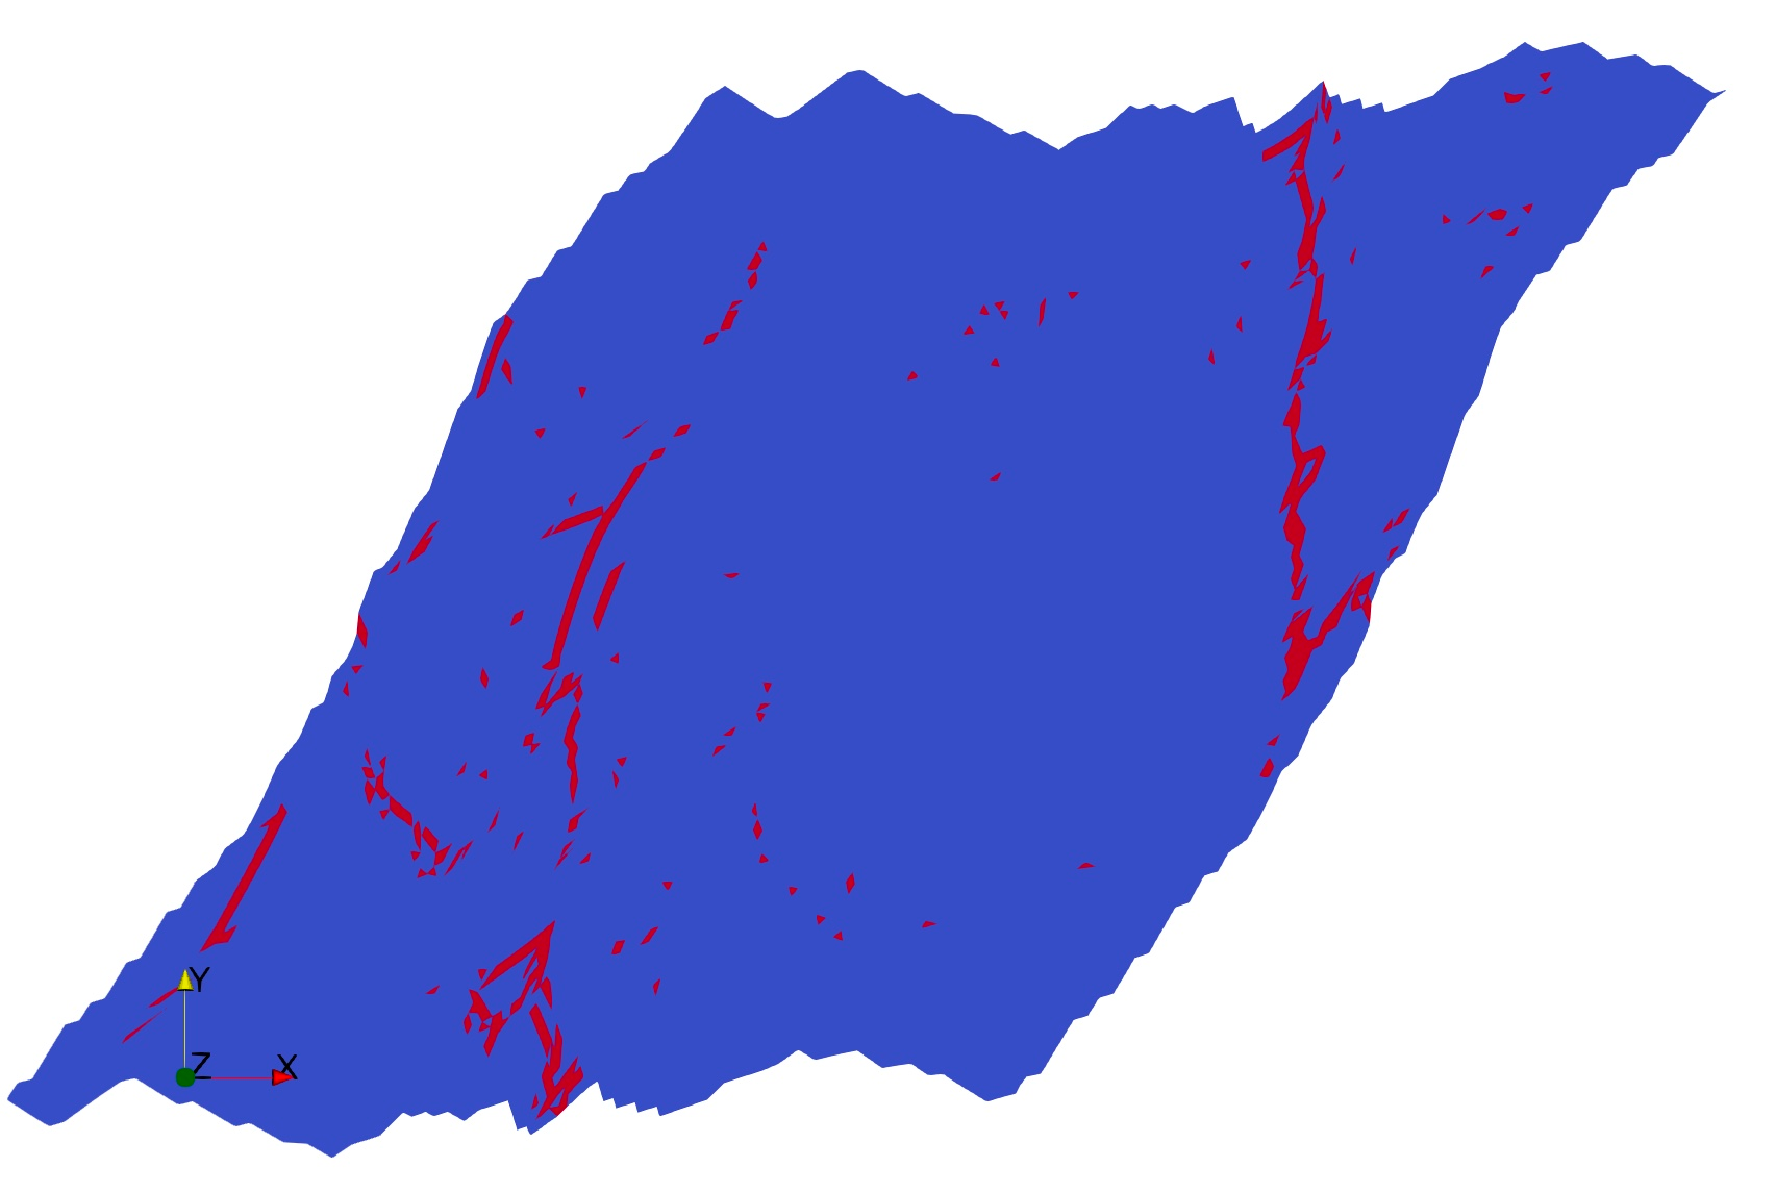
\includegraphics[scale=0.14]{./fig_sm/Fig5-b.pdf} \\
\end{tabular}
\caption{Visualizing the geometric morphology of plastically active regions during avalanche events. Domains undergoing plastic motion are colored in red. (a) In the pre-yield regime, avalanches are characterized by highly localized, spatially scattered, microscopic isolated rearrangements. (b) In the post-yield regime, deformation localizes into highly correlated, system-spanning macroscopic shear bands, where typical avalanches include the motion of grain-boundaries whose lengths are comparable to linear system size. The marked transition in structural topology—from isolated clusters to extended anisotropic bands—is directly reflected in the distinct fractal dimensions extracted from the data-collapse optimization.}
\label{sm:fig_plastified}
\end{figure}

In order to complement the 3D surface plot representations in the main text, we provide in Fig.~\ref{sm:fig_energy_histogram} an equivalent 2D configurational histograms to visualize the phase-space distribution of the local metric tensors. In the pre-yield micro-plastic regime, the system predominantly occupies three primary energy wells, corresponding to early-stage, isolated dislocation gliding along the fundamental $x$ and $y$ crystalline orientations. Conversely, in the post-yield regime, accumulated plastic strain and the macroscopic formation of shear bands cause the system to populate a much broader landscape of potential wells. Moreover, the stability envelopes derived from macroscopic acoustic tensor analysis—shown here seamlessly overlaying the histogram distributions for the first five energy wells—strictly bound the local regions surrounding each distinct well. This clear correlation demonstrates that the vast majority of mesoscopic units remain  localized inside these 'locally' stable  regions, leaving only the highly energetic, actively moving dislocation cores exposed as they traverse the unstable saddles connecting the energy minima.

\begin{figure}[htbp]
\centering
\begin{tabular}{cc}
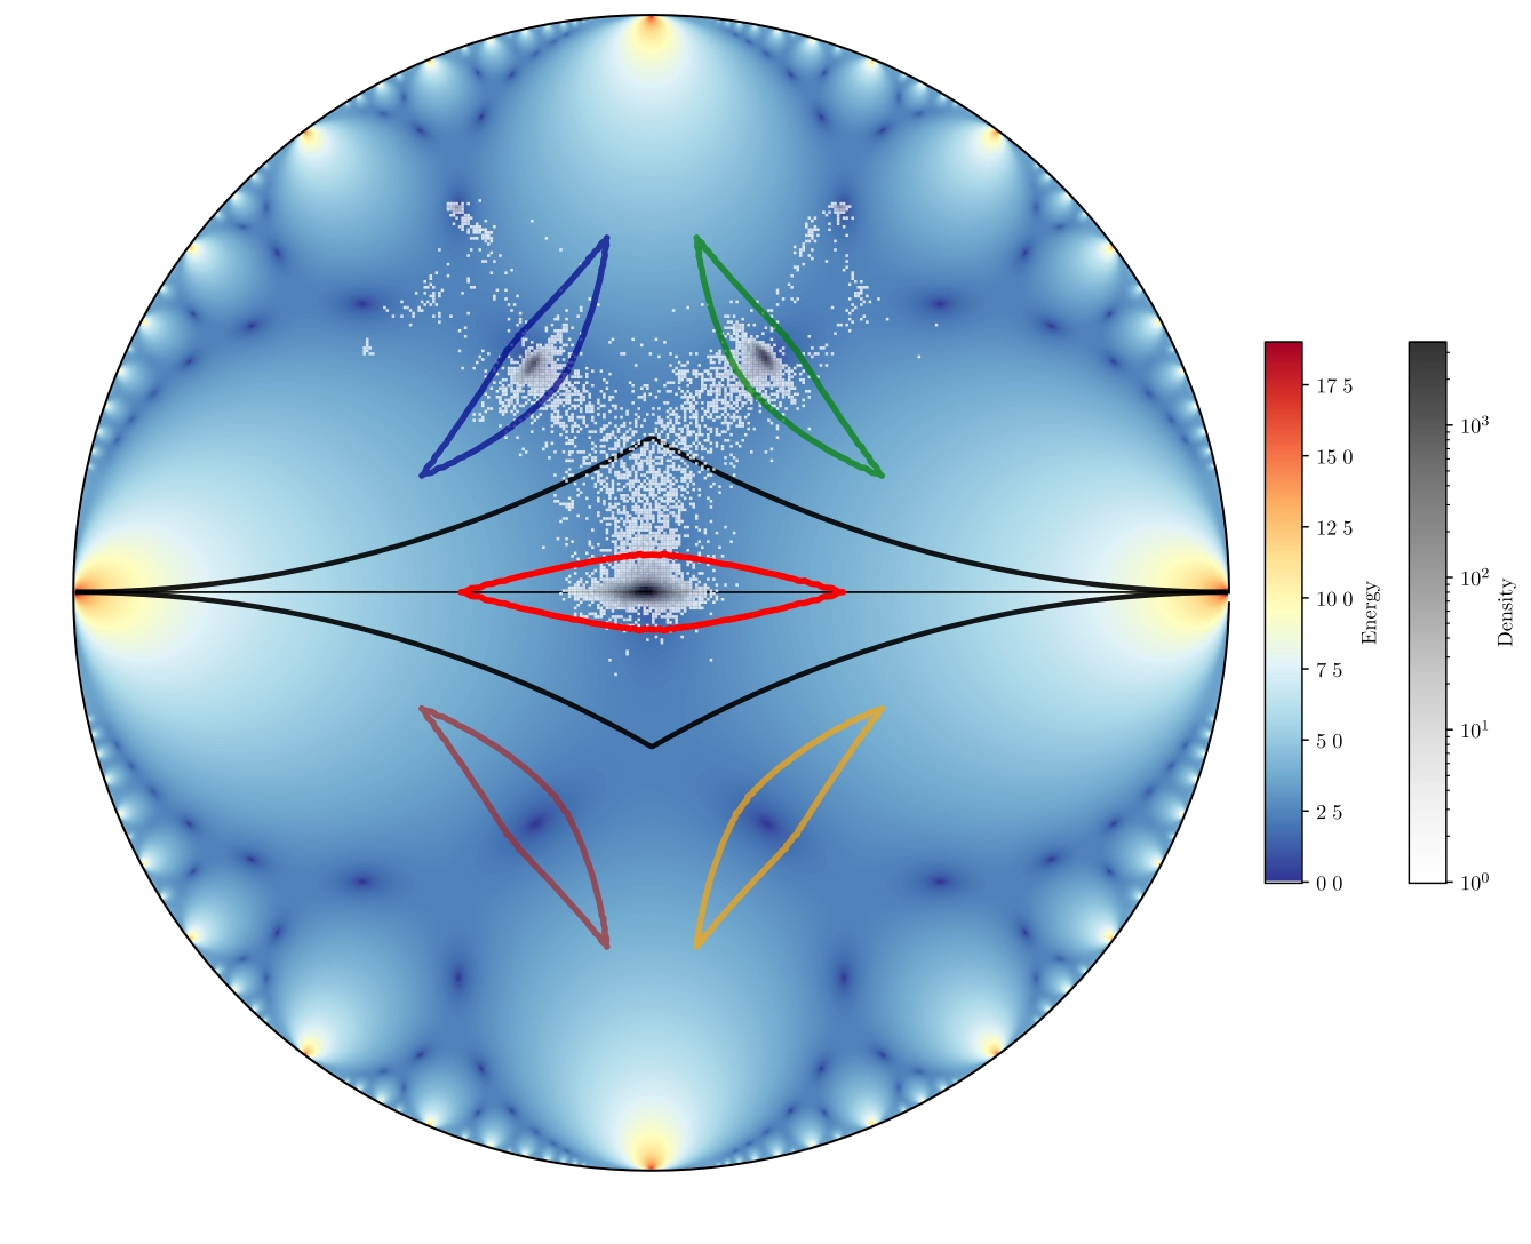
\includegraphics[scale=0.18]{./fig_sm/Fig6-a.pdf} &
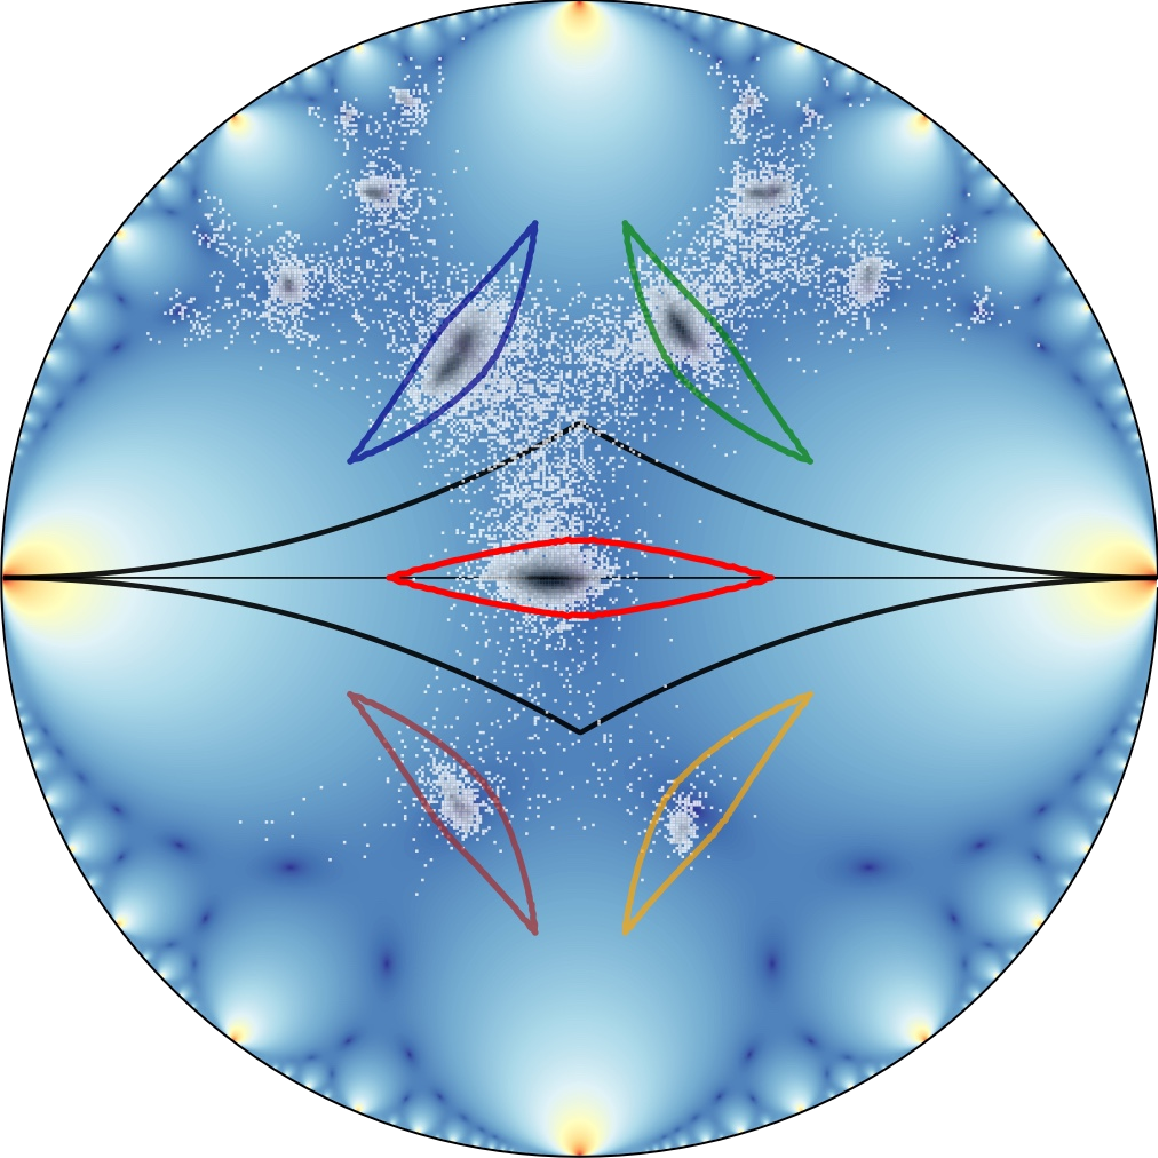
\includegraphics[scale=0.18]{./fig_sm/Fig6-b.pdf} \\
(a) Pre-yield ($\alpha \approx 0.3$) & (b) Post-yield ($\alpha \approx 0.8$) \\
\end{tabular}
\caption{2D histograms displaying the distribution of local metric tensors across the Poincaré configurational space: (a) pre-yield, (b) post-yield state. Solid lines denote stability envelops from acoustic tensor analysis encompassing the stable landscape of the first 5 wells.}
\label{sm:fig_energy_histogram}
\end{figure}

\begin{thebibliography}{11}%
\makeatletter
\providecommand \@ifxundefined [1]{%
 \@ifx{#1\undefined}
}%
\providecommand \@ifnum [1]{%
 \ifnum #1\expandafter \@firstoftwo
 \else \expandafter \@secondoftwo
 \fi
}%
\providecommand \@ifx [1]{%
 \ifx #1\expandafter \@firstoftwo
 \else \expandafter \@secondoftwo
 \fi
}%
\providecommand \natexlab [1]{#1}%
\providecommand \enquote  [1]{``#1''}%
\providecommand \bibnamefont  [1]{#1}%
\providecommand \bibfnamefont [1]{#1}%
\providecommand \citenamefont [1]{#1}%
\providecommand \href@noop [0]{\@secondoftwo}%
\providecommand \href [0]{\begingroup \@sanitize@url \@href}%
\providecommand \@href[1]{\@@startlink{#1}\@@href}%
\providecommand \@@href[1]{\endgroup#1\@@endlink}%
\providecommand \@sanitize@url [0]{\catcode `\\12\catcode `\$12\catcode
  `\&12\catcode `\#12\catcode `\^12\catcode `\_12\catcode `\%12\relax}%
\providecommand \@@startlink[1]{}%
\providecommand \@@endlink[0]{}%
\providecommand \url  [0]{\begingroup\@sanitize@url \@url }%
\providecommand \@url [1]{\endgroup\@href {#1}{\urlprefix }}%
\providecommand \urlprefix  [0]{URL }%
\providecommand \Eprint [0]{\href }%
\providecommand \doibase [0]{http://dx.doi.org/}%
\providecommand \selectlanguage [0]{\@gobble}%
\providecommand \bibinfo  [0]{\@secondoftwo}%
\providecommand \bibfield  [0]{\@secondoftwo}%
\providecommand \translation [1]{[#1]}%
\providecommand \BibitemOpen [0]{}%
\providecommand \bibitemStop [0]{}%
\providecommand \bibitemNoStop [0]{.\EOS\space}%
\providecommand \EOS [0]{\spacefactor3000\relax}%
\providecommand \BibitemShut  [1]{\csname bibitem#1\endcsname}%
\let\auto@bib@innerbib\@empty
%</preamble>
\bibitem [{\citenamefont {Parry}(1998)}]{Parry1998}%
  \BibitemOpen
  \bibfield  {author} {\bibinfo {author} {\bibfnamefont {G.~P.}\ \bibnamefont
  {Parry}},\ }\href@noop {} {\bibfield  {journal} {\bibinfo  {journal} {Arch.
  Rational Mech. Anal.}\ }\textbf {\bibinfo {volume} {145}},\ \bibinfo {pages}
  {1} (\bibinfo {year} {1998})}\BibitemShut {NoStop}%
\bibitem [{\citenamefont {Conti}\ and\ \citenamefont
  {Zanzotto}(2004)}]{Conti2004-sv}%
  \BibitemOpen
  \bibfield  {author} {\bibinfo {author} {\bibfnamefont {S.}~\bibnamefont
  {Conti}}\ and\ \bibinfo {author} {\bibfnamefont {G.}~\bibnamefont
  {Zanzotto}},\ }\href@noop {} {\bibfield  {journal} {\bibinfo  {journal}
  {Arch. Ration. Mech. Anal.}\ }\textbf {\bibinfo {volume} {173}},\ \bibinfo
  {pages} {69} (\bibinfo {year} {2004})}\BibitemShut {NoStop}%
\bibitem [{\citenamefont {Engel}(2012)}]{Engel2012}%
  \BibitemOpen
  \bibfield  {author} {\bibinfo {author} {\bibfnamefont {P.}~\bibnamefont
  {Engel}},\ }\href@noop {} {\emph {\bibinfo {title} {Geometric
  Crystallography: An Axiomatic Introduction To Crystallography}}}\ (\bibinfo
  {publisher} {Springer Science \& Business Media},\ \bibinfo {address}
  {Dordrecht},\ \bibinfo {year} {2012})\BibitemShut {NoStop}%
\bibitem [{\citenamefont {Pitteri}\ and\ \citenamefont
  {Zanzotto}(2002)}]{pitteri2002continuum}%
  \BibitemOpen
  \bibfield  {author} {\bibinfo {author} {\bibfnamefont {M.}~\bibnamefont
  {Pitteri}}\ and\ \bibinfo {author} {\bibfnamefont {G.}~\bibnamefont
  {Zanzotto}},\ }\href@noop {} {\emph {\bibinfo {title} {Continuum models for
  phase transitions and twinning in crystals}}}\ (\bibinfo  {publisher}
  {Chapman and Hall/CRC},\ \bibinfo {address} {Boca Raton},\ \bibinfo {year}
  {2002})\BibitemShut {NoStop}%
\bibitem [{\citenamefont {Baggio}\ \emph
  {et~al.}(2023{\natexlab{a}})\citenamefont {Baggio}, \citenamefont {Salman},\
  and\ \citenamefont {Truskinovsky}}]{Baggio2023}%
  \BibitemOpen
  \bibfield  {author} {\bibinfo {author} {\bibfnamefont {R.}~\bibnamefont
  {Baggio}}, \bibinfo {author} {\bibfnamefont {O.~U.}\ \bibnamefont {Salman}},
  \ and\ \bibinfo {author} {\bibfnamefont {L.}~\bibnamefont {Truskinovsky}},\
  }\href@noop {} {\bibfield  {journal} {\bibinfo  {journal} {Eur. J. Mech.
  A/Solids}\ }\textbf {\bibinfo {volume} {99}},\ \bibinfo {pages} {104897}
  (\bibinfo {year} {2023}{\natexlab{a}})}\BibitemShut {NoStop}%
\bibitem [{\citenamefont {Baggio}\ \emph
  {et~al.}(2023{\natexlab{b}})\citenamefont {Baggio}, \citenamefont {Salman},\
  and\ \citenamefont {Truskinovsky}}]{Baggio2023-qu}%
  \BibitemOpen
  \bibfield  {author} {\bibinfo {author} {\bibfnamefont {R.}~\bibnamefont
  {Baggio}}, \bibinfo {author} {\bibfnamefont {O.~U.}\ \bibnamefont {Salman}},
  \ and\ \bibinfo {author} {\bibfnamefont {L.}~\bibnamefont {Truskinovsky}},\
  }\href@noop {} {\bibfield  {journal} {\bibinfo  {journal} {Phys. Rev. E}\
  }\textbf {\bibinfo {volume} {107}},\ \bibinfo {pages} {025004} (\bibinfo
  {year} {2023}{\natexlab{b}})}\BibitemShut {NoStop}%
\bibitem [{\citenamefont {Irons}(1966)}]{Irons1966}%
  \BibitemOpen
  \bibfield  {author} {\bibinfo {author} {\bibfnamefont {B.~M.}\ \bibnamefont
  {Irons}},\ }\href@noop {} {\bibfield  {journal} {\bibinfo  {journal} {AIAA
  J.}\ }\textbf {\bibinfo {volume} {4}},\ \bibinfo {pages} {2035} (\bibinfo
  {year} {1966})}\BibitemShut {NoStop}%
\bibitem [{\citenamefont {Bramble}\ and\ \citenamefont
  {Zl\'{a}mal}(1970)}]{Bramble1970-oq}%
  \BibitemOpen
  \bibfield  {author} {\bibinfo {author} {\bibfnamefont {J.~H.}\ \bibnamefont
  {Bramble}}\ and\ \bibinfo {author} {\bibfnamefont {M.}~\bibnamefont
  {Zl\'{a}mal}},\ }\href@noop {} {\bibfield  {journal} {\bibinfo  {journal}
  {Math. Comp.}\ }\textbf {\bibinfo {volume} {24}},\ \bibinfo {pages} {809}
  (\bibinfo {year} {1970})}\BibitemShut {NoStop}%
\bibitem [{\citenamefont {Bochkanov}\ and\ \citenamefont
  {Bystritsky}(2013)}]{Bochkanov2013-lk}%
  \BibitemOpen
  \bibfield  {author} {\bibinfo {author} {\bibfnamefont {S.}~\bibnamefont
  {Bochkanov}}\ and\ \bibinfo {author} {\bibfnamefont {V.}~\bibnamefont
  {Bystritsky}},\ }\href@noop {} {\bibfield  {journal} {\bibinfo  {journal}
  {Available from: www alglib net}\ } (\bibinfo {year} {2013})}\BibitemShut
  {NoStop}%
\bibitem [{\citenamefont {Sanderson}\ and\ \citenamefont
  {Curtin}(2016)}]{Sanderson2016-ht}%
  \BibitemOpen
  \bibfield  {author} {\bibinfo {author} {\bibfnamefont {C.}~\bibnamefont
  {Sanderson}}\ and\ \bibinfo {author} {\bibfnamefont {R.}~\bibnamefont
  {Curtin}},\ }\href@noop {} {\bibfield  {journal} {\bibinfo  {journal} {J Open
  Source Softw}\ }\textbf {\bibinfo {volume} {1}},\ \bibinfo {pages} {26}
  (\bibinfo {year} {2016})}\BibitemShut {NoStop}%
\bibitem [{\citenamefont {Fishman}\ \emph {et~al.}(2022)\citenamefont
  {Fishman}, \citenamefont {White},\ and\ \citenamefont
  {Stoudenmire}}]{Fishman2022-nj}%
  \BibitemOpen
  \bibfield  {author} {\bibinfo {author} {\bibfnamefont {M.}~\bibnamefont
  {Fishman}}, \bibinfo {author} {\bibfnamefont {S.}~\bibnamefont {White}}, \
  and\ \bibinfo {author} {\bibfnamefont {E.}~\bibnamefont {Stoudenmire}},\
  }\href@noop {} {\bibfield  {journal} {\bibinfo  {journal} {SciPost Phys.
  Codebases}\ ,\ \bibinfo {pages} {004}} (\bibinfo {year} {2022})}\BibitemShut
  {NoStop}%
\end{thebibliography}%




\end{document}


%https://www.scirp.org/journal/paperinformation.aspx?paperid=108300
%
%https://www.scientific.net/KEM.725.636